% Version 0; preprint format; Outline of paper II by Song Huang
% Version 1; preprint format; Edited by Jenny Greene
% Version 2; preprint format; Edited by Song Huang

\documentclass[a4paper,fleqn,usenatbib]{mnras}

% Packages
\usepackage{deluxetable}
\usepackage{newtxtext,newtxmath}
\usepackage[T1]{fontenc}
\usepackage{ae,aecompl}
\usepackage{amssymb, amsmath}
\usepackage{graphicx}
\usepackage{natbib}
\usepackage{url}
\usepackage{hyperref}
\usepackage{float}
\usepackage[usenames, dvipsnames]{color}

% Package Settings
\hypersetup{colorlinks=true,
            citecolor=cyan,
            linkcolor=cyan,
            filecolor=magenta,      
            urlcolor=cyan}
\urlstyle{same}

% Figure extention
\DeclareGraphicsExtensions{.pdf,.png,.jpg}

%%%%%%%%%%%%: User Defined Commands %%%%%%%%%%%%

% Song Huang's definition 
\def\arcsec{{\prime\prime}}
\def\arcmin{{\prime}}
\def\degree{{\circ}}
\def\h{\hskip -3 mm}
\def\aa{{A\&A}}
\def\aas{{ A\&AS}}
\def\aj{{AJ}}
\def\al{$\alpha$}
\def\bet{$\beta$}
\def\amin{$^\prime$}
\def\annrev{{ARA\&A}}
\def\apj{{ApJ}}
\def\apjs{{ApJS}}
\def\asec{$^{\prime\prime}$}
\def\deg{$^{\circ}$}
\def\ddeg{{\rlap.}$^{\circ}$}
\def\dsec{{\rlap.}$^{\prime\prime}$}
\def\cc{cm$^{-3}$}
\def\flamb{erg s$^{-1}$ cm$^{-2}$ \AA$^{-1}$}
\def\flux{erg s$^{-1}$ cm$^{-2}$}
\def\fnu{erg s$^{-1}$ cm$^{-2}$ Hz$^{-1}$}
\def\hst{{\textit{HST}}}
\def\kms{km s$^{-1}$}
\def\lamb{$\lambda$}
\def\lax{{$\mathrel{\hbox{\rlap{\hbox{\lower4pt\hbox{${\sim}$}}}\hbox{$<$}}}$}}
\def\gax{{$\mathrel{\hbox{\rlap{\hbox{\lower4pt\hbox{${\sim}$}}}\hbox{$>$}}}$}}
\def\simlt{\lower.5ex\hbox{$\; \buildrel < \over {\sim} \;$}}
\def\simgt{\lower.5ex\hbox{$\; \buildrel > \over {\sim} \;$}}
\def\micron{{$\mu$m}}
\def\mnras{{MNRAS}}
\def\nat{{Nature}}
\def\pasp{{PASP}}
\def\perang{\AA$^{-1}$}
\def\peryr{yr$^{-1}$}
\def\reference{\noindent\pp}
\def\refindent{\par\noindent\parskip=2pt\hangindent=3pc\hangafter=1 }
\def\sb{mag~arcsec$^{-2}$}
\def\lsun{$L_\odot$} 
\def\msun{$M_\odot$}
\def\sigs{$\sigma_*$}
\newcommand{\lt}{<}
\newcommand{\gt}{>}

\def\etal{{\ et al.~}}
\def\galfit{{\tt GALFIT}}
\def\ser{{S\'{e}rsic\ }}
\def\redm{\texttt{redMaPPer}}
\def\cmodel{\texttt{cModel}}
% Samples
\def\rbcg{\texttt{cenHighMh}}
\def\nbcg{\texttt{cenLowMh}}
\def\redbcg{{$\lambda \ge 30$}}
\def\nonbcg{{$\lambda < 20$}}
% Mass related 
\def\mstar{{$M_{\star}$}}
\def\mhalo{{$M_{\mathrm{halo}}$}}
\def\logms{{$\log (M_{\star}/M_{\odot})$}}
\def\logmh{{$\log (M_{\mathrm{halo}}/M_{\odot})$}}

\def\minn{{$M_{\star,10\mathrm{kpc}}$}}
\def\meff{{$M_{\star,15\mathrm{kpc}}$}} 
\def\mtot{{$M_{\star,100\mathrm{kpc}}$}}
\def\mout{{$M_{\star,150\mathrm{kpc}}$}}
\def\mmax{{$M_{\star,\mathrm{Max}}$}}
\def\mgama{{$M_{\star,\mathrm{GAMA}}$}}
\def\mcmodel{{$M_{\star,\mathrm{cModel}}$}}

\def\logminn{{$\log (M_{\star,10\mathrm{kpc}}/M_{\odot})$}}
\def\logmtot{{$\log (M_{\star,100\mathrm{kpc}}/M_{\odot})$}}
\def\logmout{{$\log (M_{\star,150\mathrm{kpc}}/M_{\odot})$}}
\def\logmmax{{$\log (M_{\star,\mathrm{Max}}/M_{\odot})$}}
\def\logmgama{{$\log (M_{\star,\mathrm{GAMA}}/M_{\odot})$}}
\def\logmcmodel{{$\log (M_{\star,\mathrm{cModel}}/M_{\odot})$}}

\def\m2l{{$M_{\star}/L_{\star}$}}
\def\s2n{{$\mathrm{S}/\mathrm{N}$}}
\def\mden{{$\mu_{\star}$}}

\def\insitu{{\textit{in situ}}}
\def\exsitu{{\textit{ex situ}}}

% Commenting:
\newcommand{\xxx}[1]{\textcolor{red}{\textbf{XXX}}}
\newcommand{\todo}[1]{\textcolor{red}{\textbf{TODO:~#1}}}
\newcommand{\plan}[1]{\textcolor{cyan}{#1}}
\newcommand{\addref}{{\textcolor{red}{REF}}}
\newcommand{\note}[2]{\textcolor{blue}{\textbf{[Comment (#1): #2]}}}
\newcommand{\song}[1]{\textcolor{magenta}{\textbf{[Song: #1]}}}
\newcommand{\alexie}[1]{\textcolor{blue}{\textbf{[Alexie: #1]}}}
\newcommand{\jenny}[1]{\textcolor{Bittersweet}{\textbf{[Jenny: #1]}}}
\newcommand{\kevin}[1]{\textcolor{green}{\textbf{[Kevin: #1]}}}
\newcommand{\update}[1]{\textcolor{PineGreen}{#1}}

%% ------------------------------------------------------------------------------------ %% 
%% Title and Affiliations 
%% ------------------------------------------------------------------------------------ %% 

\title[Structure and Environment of Massive Galaxies]{
       A Detection of the Environmental Dependence of the Stellar Profiles and haloes
       of Massive Central Galaxies}

\author[S. Huang et al.]{
        Song Huang,$^{1,2}$\thanks{E-mail: song.huang@ipmu.jp (SH)}
        Alexie Leauthaud,$^{2,1}$
        Jenny Greene,$^{4}$
        Kevin Bundy,$^{3,1}$
        \newauthor
        Yen-Ting Lin,$^{5}$
        Masayuki Tanaka,$^{6}$
        Rachel Mandelbaum,$^{7}$
        Satoshi Miyazaki,$^{5,8}$
        \newauthor
        Yutaka Komiyama$^{5,8}$
        \\
        $^{1}$Kavli-IPMU, The University of Tokyo Institutes for Advanced Study, 
              the University of Tokyo (Kavli IPMU, WPI), Kashiwa 277--8583, Japan\\
        $^{2}$Department of Astronomy and Astrophysics, University of California 
              Santa Cruz, 1156 High St., Santa Cruz, CA 95064, U.S.A\\
        $^{3}$UCO/Lick Observatory, University of California, Santa Cruz,
              1156 High Street, Santa Cruz, CA 95064, USA\\
        $^{4}$Department of Astrophysical Sciences, Peyton Hall,
              Princeton University, Princeton, NJ 08540, USA \\
        $^{5}$National Astronomical Observatory of Japan, 2--21--1 Osawa, Mitaka, 
              Tokyo 181--8588, Japan\\
        $^{6}$Academia Sinica Institute of Astronomy and Astrophysics, 
              P.O. Box 23--141, Taipei 10617, Taiwan\\
        $^{7}$McWilliams Center for Cosmology, Department of Physics, 
              Carnegie Mellon University, Pittsburgh, PA 15213, USA\\
        $^{8}$SOKENDAI (The Graduate University for Advanced Studies), Mitaka,
              Tokyo, 181--8588, Japan
        }   
%% ------------------------------------------------------------------------------------ %% 
\date{Accepted XXX. Received YYY; in original form ZZZ}        
\pubyear{2017}                                  
  
%% ------------------------------------------------------------------------------------ %% 
%% Header and Version 
%% ------------------------------------------------------------------------------------ %% 

\begin{document}

\label{firstpage}
\pagerange{\pageref{firstpage}--\pageref{lastpage}}

\maketitle

%% ------------------------------------------------------------------------------------ %% 
%% Abstract and Keywords 
%% ------------------------------------------------------------------------------------ %% 

\begin{abstract} 
    
    We use ${\sim}100$ deg$^2$ of deep ($>28.5$ \sb{} in $i$-band), high-quality 
    (0.6\asec seeing) imaging data from the Hyper Suprime-Cam (HSC) survey 
    to investigate the halo mass dependence of the surface mass density profiles 
    and outer stellar envelopes of massive galaxies. 
    Our sample consists of ${\sim}7000$ massive (\mstar{}$\geq 11.5$) central galaxies 
    at $0.3 < z < 0.5$. 
    The depth of the HSC survey reaches ${\sim}4$ magnitudes fainter than SDSS and 
    enables us to directly trace stellar mass distributions to 100 kpc without 
    requiring stacking. 
    For the first time, we conclusively show that at fixed stellar mass, massive central 
    galaxies display mass density profiles that are not self similar and which 
    present subtle but systematic differences that correlate with \mhalo{}. 
    On average, massive central galaxies in more massive haloes have shallower inner 
    stellar mass density profiles (within ${\sim}10$-$20$ kpc) and more prominent outer 
    envelopes. 
    These differences translate into a clear environmental dependence of the mass-size 
    relation: central galaxies in more massive haloes have larger $R_{\mathrm{50}}$ 
    at fixed \mtot{}. 
    Shallow imaging will miss light at the outskirts of galaxies and this has an 
    important impact on measurements of the galaxy mass function. 
    Furthermore, because galaxies in larger haloes have more extended envelopes, 
    the amount of light that is missed will be halo mass dependent. 
    Finally, at fixed total stellar mass, there is a large (but continuous) diversity 
    in the amplitude of stellar profiles at 100 kpc. 
    We argue that ``cD'' galaxies represent the tail end of a distribution and 
    are not a distinct class of massive galaxies. 
    Our results are broadly consistent with the two phase formation scenario of 
    massive galaxies in which outer envelopes are built up at late times from the 
    accretion of small systems. 
    Our mass profiles are provided in a convenient tabulated format in order to 
    facilitate comparisons with predictions from numerical simulations of galaxy 
    formation. 
    \song{This is the abstract of old draft, need some works}
    
\end{abstract}

\begin{keywords}
    galaxies: elliptical and lenticular, cD --
    galaxies: formation --
    galaxies: photometry -- 
    galaxies: structure -- 
    galaxies: surveys
\end{keywords}


%% ------------------------------------------------------------------------------------ %% 
%% Main Text
%% ------------------------------------------------------------------------------------ %% 


%% ------------------------------------------------------------------------------------ %% 
%% Introduction 
%% ------------------------------------------------------------------------------------ %% 

\section{Introduction}
    \label{sec:intro}
    
    One of the most intriguing observations of high-redshift galaxies from the last 
    decade has been the dramatic structural transformation in massive quiescent 
    galaxies \citep[e.g.][]{Trujillo2006, vanDokkum2008, Cimatti2008, Damjanov2009, 
    vanderWel2011, Szomoru2012, Patel2013} from $z \approx 2$ to the present. 
    These observations suggest that the progenitors of $z{\sim} 0$ massive early-type 
    galaxies (ETGs) need to increase their effective radius ($R_{\rm e}$) by factor 
    of 2--4 in the last 10 Gyrs (e.g. \citealt{Newman2012, vdWel2014}).
    They have led to a ``two-phase'' scenario for the formation of massive ETGs 
    (e.g. \citealt{Oser2010, Oser2012}),
    in which galaxies form a compact central region through highly dissipative 
    processes (e.g. gas-rich merger or cold gas-accretion; 
    \citealt{Hopkins2008, Dekel2009}) and then assemble their extended stellar 
    haloes via dry mergers 
    \citep[e.g,][]{Naab2006, Khochfar2006, Oser2010, Oser2012}, which allows for 
    significant growth at late times. 
    Meanwhile, progenitor bias, which proposes that larger ETGs were quenched more 
    recently, could also contribute to the apparent size growth, although its 
    important is under argument (e.g. \citealt{Newman2012, Carollo2013, 
    Poggianti2013, Belli2015, Keating2015, Fagioli2016}). 
    
    Several previous works have tested the two-phase formation scenario 
    observationally using galaxies at low redshift, looking at their surface 
    brightness of mass density profiles (e.g. \citealt{Huang2013a, Huang2013b, 
    Oh2017}, optical color gradients (e.g. \citealt{LaBarbera2010, LaBarbera2012}), 
    and stellar population gradients \citep[e.g.,][]{Coccato2010, Coccato2011, 
    Greene2015, Barbosa2016}. 
    These observations are generally consistent with the two-phase scenario, 
    but this picture still face many challenges.
    One of the most outstanding issues is the extent to which, at fixed stellar mass, 
    the accreted fraction depends on the surrounding dark matter halo mass. 
    
    According to this two-phase formation scenario, the late time growth of massive 
    ETGs is intrinsically tied to the growth of their host dark matter haloes 
    (e.g. \citealt{Leauthaud2012, Behroozi2013, Shankar2013}). 
    Massive ETGs that live at the center of more massive haloes should experience 
    different assembly and should be subject to higher merger rate compared to 
    ETGs with similar \mstar{} that live in less massive dark matter haloes. 
    A natural prediction of this picture is therefore that the structures of 
    massive ETGs should depend on their ``environment''\footnote{There are 
    different definitions of ``environment'' in the literature.  
    In this work, we use ``environment'' and halo mass interchangeably.}.
    For instance, models based on two-phase scenario predict that the well-know 
    stellar mass--effective radius relation for ETGs (\mstar{}--$R_{\rm e}$ relation; 
    e.g., \citealt{Shen2003, Guo2009}) should show environmental dependence: the 
    $R_{\rm e}$ of massive ETGs in more massive haloes should be larger than those 
    in less massive haloes at fixed \mstar{} 
    (e.g. \citealt{Shankar2013, Shankar2014}).
    Yet, solid evidence of this effect at low redshift is still missing 
    (e.g. \citealt{Nair2010, HCompany13}; but also see \citealt{Yoon2017}).
    
    %However, while hints of an environmental dependence in the mass-size relation have 
    %been spotted at high-$z$ (e.g. \citealt{Papovich2012, Lani2013, Delaye2014}; but 
    %also see \citealt{Rettura2010}). 
    
	% Song: Actually the Illustris paper suggests that, for massive galaxies, 
	%       even the inner region is dominated by accreted stars. 
	
    To seriously test the environmental dependence of structure in massive ETGs 
    requires highly sensitive observations extending beyond the inner region of these 
    galaxies to truly probe the material accreted at late times. 
    This is very challenging observation as the surface brightness drops rapidly 
    with radius in massive ETGs. 
    
    In \citet[][Paper I hereafter]{hscMassiveI}, we showed that the deep, 
    multi-band images from the Subaru Strategic Program (SSP; \citealt{HSC-SSP,
    HSC-DR1}) using Hyper Suprime-Cam (HSC; \citealt{Miyazaki2012}, 
    Miyazaki in~prep.) allows us to extract robust surface stellar
    mass density (\mden{}) profiles for {\it individual} massive galaxies 
    at $0.3 < z < 0.5$ out to 100 kpc. 
    In Paper I, we exploited this sensitivity to show that the \mden{} profiles 
    and the shapes of the stellar haloes of massive ETGs has a clear \mstar{} 
    dependence. 
    And the fraction of accreted stars residing in the extended envelope increases
    with the total \mstar{} of the galaxy.
    
    In this paper, we explore how the extended stellar halo in massive central galaxies
    depends on dark matter halo mass with the help of HSC images of a large sample 
    of massive ETGs and the \redm{} cluster catalog (e.g.\ \citealt{Rykoff2014}; 
    \citealt{Rozo2015b}; please see \S \ref{sec:data} for details)
    
    This paper is organized as follows. 
    \S \ref{sec:data} briefly introduce the sample selection and data reduction 
    processes.  
    Please refer to \citet{hscMassiveI} for more technical details.
    Our main results are presented in \S \ref{sec:result} and discussed in 
    \S \ref{sec:discussion}. 
    \S \ref{sec:summary} presents our summary and conclusions.

    Magnitudes use the AB system (\citealt{Oke1983}), and are corrected for Galactic 
    extinction using calibrations from \citet{Schlafly11}.
    In this work, we assume $H_0$ = 70~km~s$^{-1}$ Mpc$^{-1}$, ${\Omega}_{\rm m}=0.3$, 
    and ${\Omega}_{\rm \Lambda}=0.7$.
    Stellar mass is denoted \mstar{} and has been derived using a Chabrier Initial Mass 
    Function (IMF; \citealt{Chabrier2003}).   
      
    Halo mass is defined as $M_{\rm 200b}$ as 
    $M_{\rm 200b}\equiv M(<r_{\rm 200b})=200\bar{\rho} 
    \frac{4}{3}\pi r_{\rm 200b}^3$ where $r_{\rm 200b}$
    is the radius at which the mean interior density is equal to 200 times
    the mean matter density ($\bar{\rho}$). 
    
    As in \citet{hscMassiveI}, we do not try to separate any potential ``intra-cluster''
    component (ICL; e.g. \citealt{Carlberg1997, Lin2004, Gonzalez2005, Mihos2005}) from 
    massive galaxies in our sample for both technical and scientific reasons.  
%% ------------------------------------------------------------------------------------ %% 

%% ------------------------------------------------------------------------------------ %% 
  \begin{figure*}
      \centering 
      \includegraphics[width=\textwidth]{fig/redbcg_m100_m10_compare}
      \caption{
          Three-color images for a subsample of massive galaxies at $z{\sim}0.4$. 
          All of these massive galaxies have very similar \mstar{} within a 10 kpc 
          elliptical aperture 
          ($11.2<\log (M_{\star,10\ \mathrm{kpc}}/M_{\odot})<11.3$). 
          The dash-line circle at the top-left figure indicates $R=$10 kpc.
          These galaxies are rank-ordered from top to bottom and from left to right 
          by their \mstar{} within a 100 kpc elliptical aperture which varies 
          from $10^{11.2} M_{\odot}$ to $10^{11.7} M_{\odot}$. 
          At fixed ``inner'' mass (\minn{}), massive galaxies display significant
          diversity in their outer profiles. 
          Red boxes indicate galaxies from dark matter haloes that are more massive 
          than ${\sim} 10^{14.0} M_{\odot}$. 
          }
      \label{fig:m100_m10_color}
  \end{figure*}
%% ------------------------------------------------------------------------------------ %% 

%% ------------------------------------------------------------------------------------ %% 
  \begin{figure*}
      \centering 
      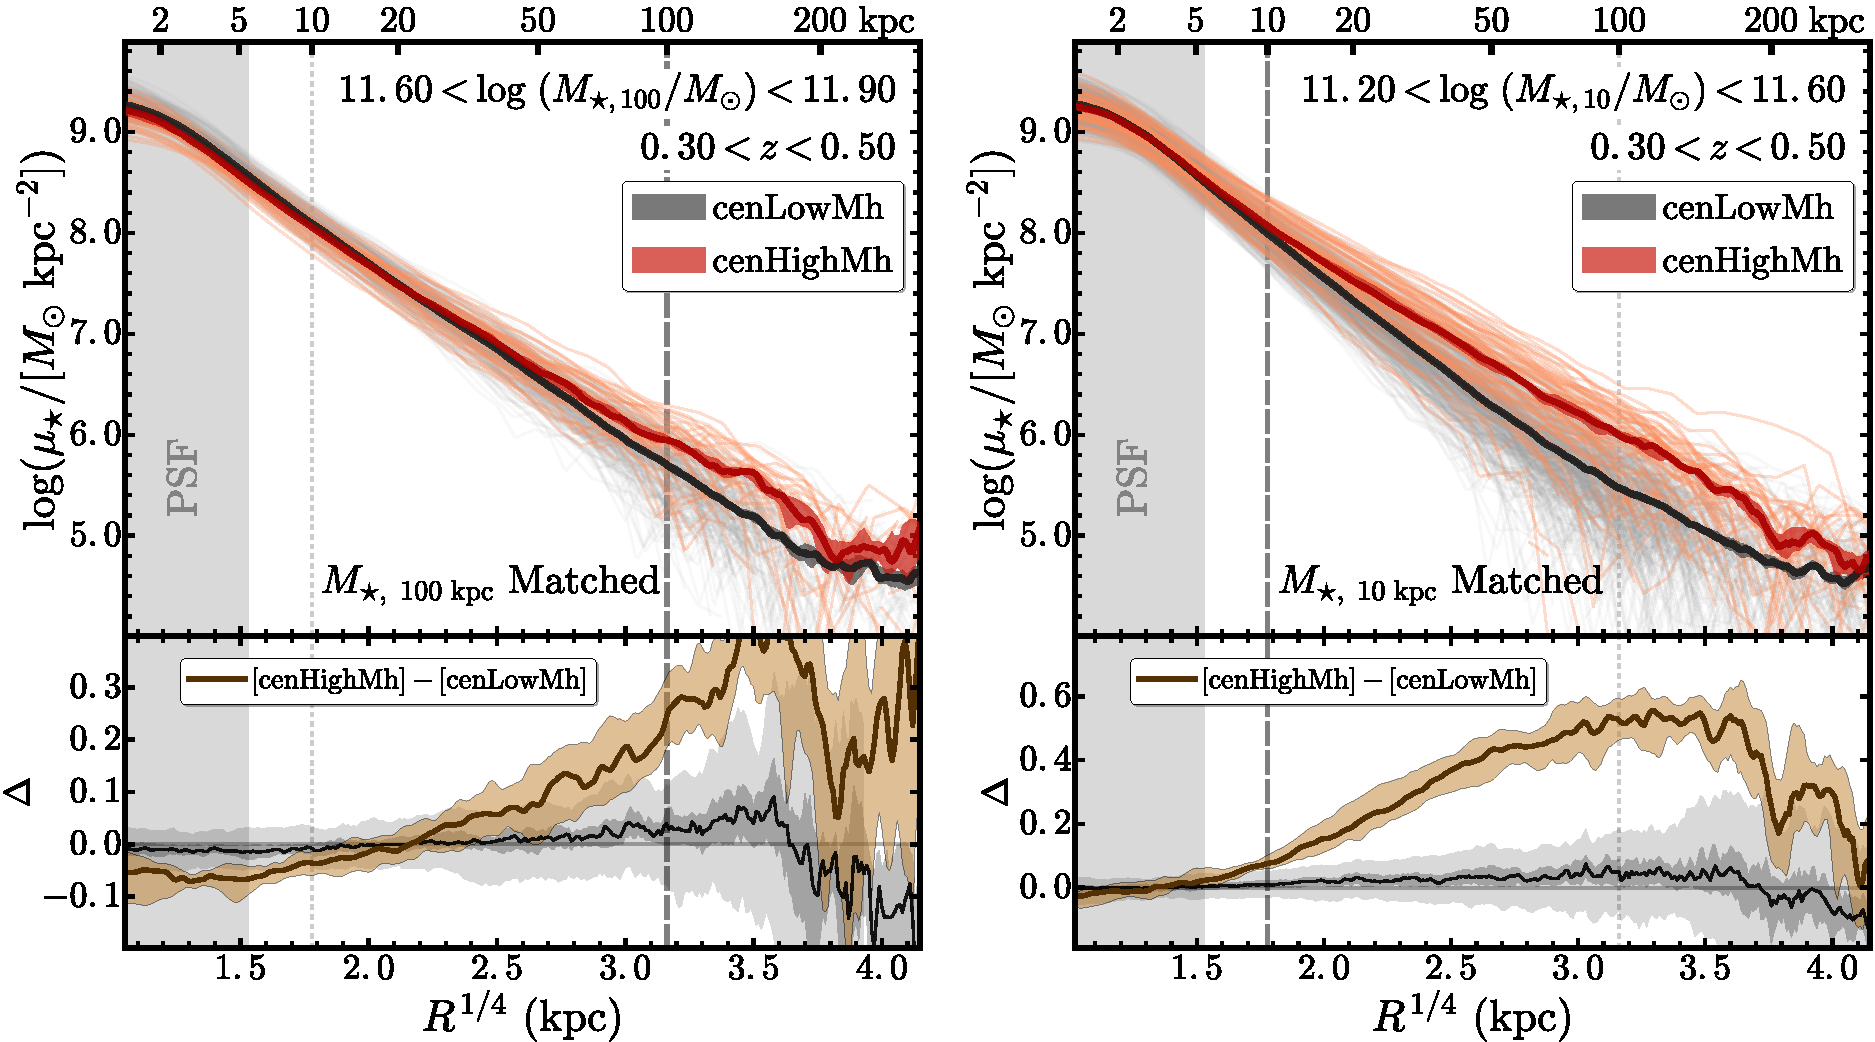
\includegraphics[width=\textwidth]{fig/redbcg_prof_1}
      \caption{
          The environmental dependence of the stellar mass profiles of massive central 
          galaxies. 
          The left panel corresponds to samples matched by ``total'' stellar mass 
          (\mtot{}). 
          The right panel corresponds to samples matched by ``core-mass'' (\minn{}). 
          Orange and red lines correspond to central galaxies living in haloes with 
          \logmh{} $\geq 14.2$. 
          Black and grey correspond to central galaxies living in haloes with 
          \logmh{} $\leq 14.0$. 
          Thin lines show the profiles of individual galaxies while thick lines show 
          the median profile. 
          The uncertainty on the median profile is given by the shaded region and is 
          computed via bootstrap resampling. 
          The brown line in the bottom panels show the relative difference between 
          two median profiles 
          ($\Delta = \log(\mu_{\star, \mathrm{cenHighMh}}) - 
          \log(\mu_{\star, \mathrm{cenLowMh}})$). 
          Errors on the difference between the two profiles is computed via bootstrap 
          too. 
          The grey shaded regions show a Monte Carlo test to asses how likely is it to 
          obtain $\Delta$ from random sub-samples of the data. 
          To compute the grey shaded regions, we first mix the two samples 
          (\rbcg{} and \nbcg{}), then draw sub-samples of galaxies from the mixed 
          population and compute $\Delta$ in the same fashion as for our fiducial signal. 
          We repeat this process 5000 times.  
          The dark-grey shaded region (light-grey shaded region) shows the 1-$\sigma$ 
          (3-$\sigma$) fluctuations in $\Delta$ from these 5000 draws.
          }
      \label{fig:prof_1} 
  \end{figure*}
%% ------------------------------------------------------------------------------------ %% 

%% ------------------------------------------------------------------------------------ %% 
  \begin{figure*}
      \centering 
      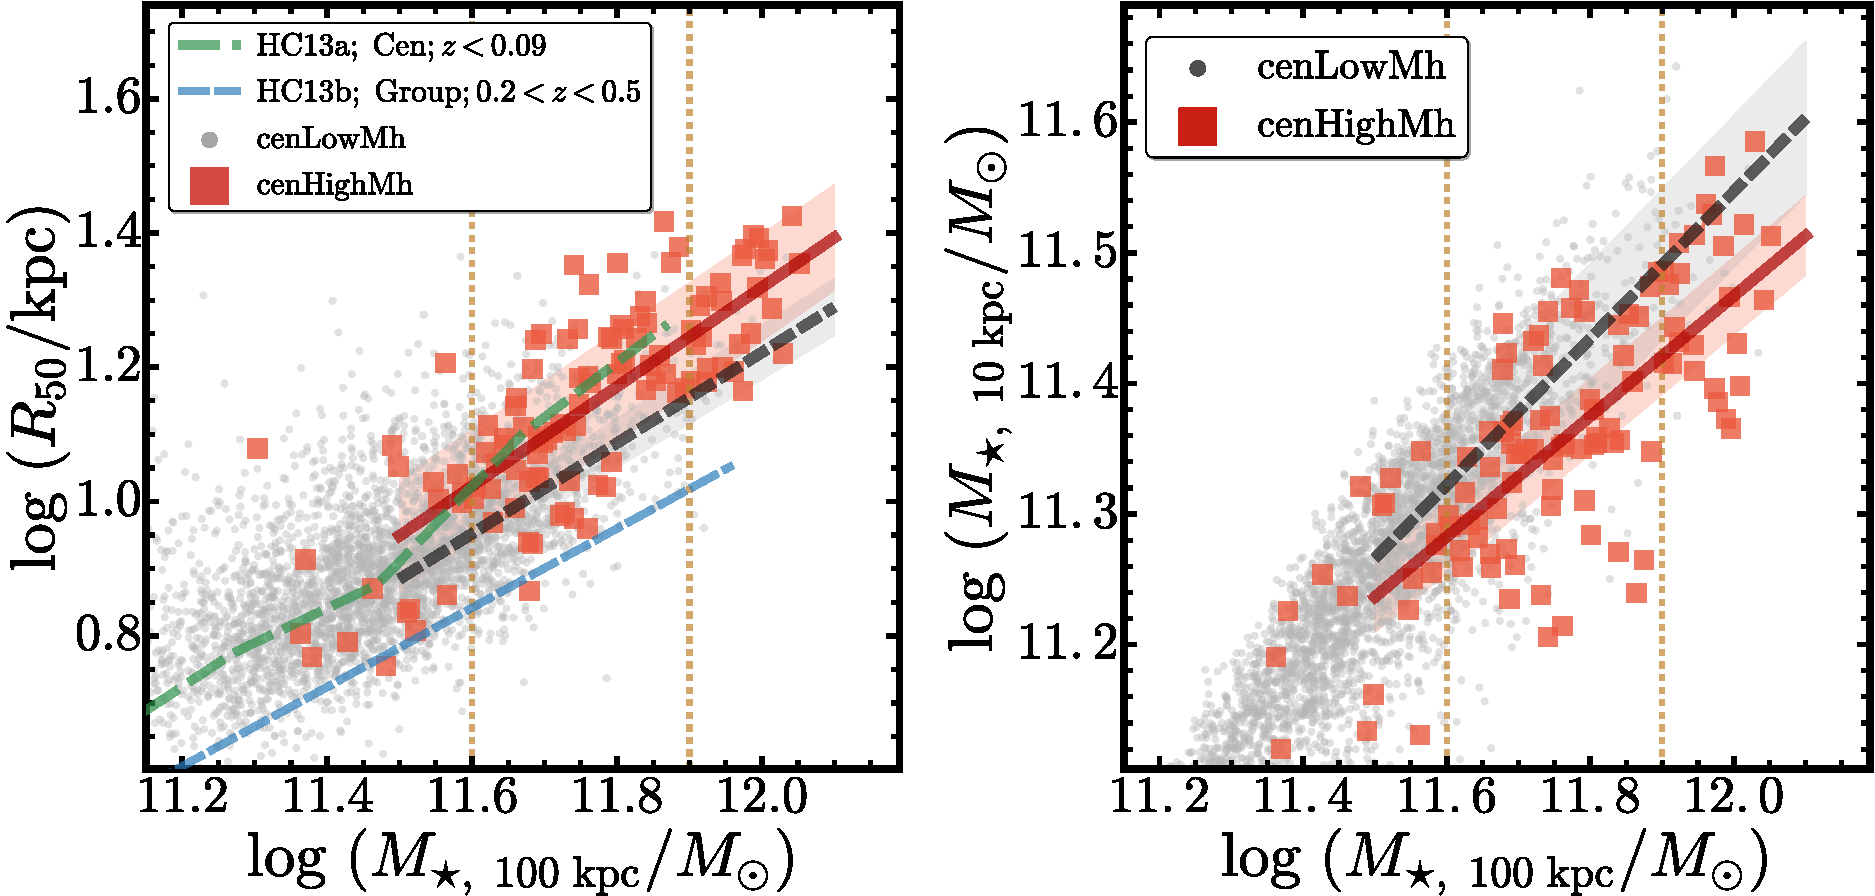
\includegraphics[width=\textwidth]{fig/redbcg_scaling_relation}
      \caption{
          \textbf{Left}: The mass-size relations for \rbcg{} (orange squares) and 
          \nbcg{} (grey dots) galaxies. 
          Two vertical lines highlight our $11.6<$ \logms{} $<11.9$ mass bin. 
          The red solid line shows the best fit mass-size relation for \rbcg{} and the 
          grey dashed line shows the best fit relation for \nbcg{}. 
          Shaded regions in lighter colors show the 1-$\sigma$ uncertainties
          from MCMC sampling.  
          The green dashed line shows the mass-size relation for nearby central 
          galaxies in massive groups from \citet{HCompany13}. 
          \textbf{Right:} The relations between \mtot{} and \minn{} for the 
          \rbcg{} and \nbcg{} galaxies, along with the best-fit scaling relations for 
          both samples.
          }
      \label{fig:scaling_relation} 
  \end{figure*}
%% ------------------------------------------------------------------------------------ %% 

%% ------------------------------------------------------------------------------------ %% 
%% Sample Selection and Data Reduction
%% ------------------------------------------------------------------------------------ %% 
\section{Sample Selection and Data Reduction}
    \label{sec:data}
    
    The sample selection and data reduction processes are described in detail in 
    Paper I. 
    Here we include a short summary for completeness.
    
    This work makes use of the imaging data from the internal data release 
    \texttt{S15B}, which is very similar to the Public Data Release 1 
    (\citealt{HSC-DR1} and covers ${\sim} 110$ deg$^2$ in all five-band ($grizy$) to 
    the required depth. 
    These images are reduced by \texttt{hscPipe 4.0.2}, a derivative of the 
    Large Synoptic Survey Telescope (LSST) pipeline (e.g.\ \citealt{Juric2015}; 
    \citealt{Axelrod2010}), modified for HSC (\citealt{HSC-PIPE}).
    The pixel scale of the reduced image is $0.168$\asec{}.
    We use the $i$-band image for extracting surface brightness profiles.    
    The HSC $i$-band image is typically 3--4 mag deeper than the SDSS one in surface 
    brightness limit and has superb seeing condition (mean FWHM$=0.6$\asec{}).
    
    In Paper~I, we select large sample of massive galaxies with either spectroscopic 
    redshift or reliable ``red-sequence'' photometric redshift (\citealt{Rykoff2014}) 
    at $0.3<z<0.5$. 
    Within this redshift range, we have large enough volume to achieve reasonable 
    statistics at very high \mstar{} end, can spatially resolve the inner $\sim 5$ 
    kpc of massive galaxies ($1.0^{\arcsec}$ corresponds to 4.4 and 6.1 kpc at 
    $z=0.3$ and 0.5), and can safely ignore any structural evolution. 
    We derive $i$-band surface brightness profiles out to 100 kpc after carefully 
    masking out any surrounding contaminations and correcting the background 
    subtraction. 
    We use the broadband spectral energy distributions (SED) fitting code 
    \texttt{iSEDFit}\footnote{http://www.sos.siena.edu/~jmoustakas/isedfit/} 
    (\citealt{Moustakas13}) to measure the average \m2l{} and $k$--correction of 
    these galaxies using five-band forced \cmodel{} magnitudes from \texttt{hscPipe}.
    \citet{Chabrier2003} IMF, Flexible Stellar Population 
    Synthesis\footnote{http://scholar.harvard.edu/cconroy/sps-models}
    (FSPS; \texttt{v2.4}; \citealt{FSPS}, \citealt{Conroy2010}) model, 
    \citet{Calzetti2000} extinction law, simple delayed-$\tau$ model for star 
    formation history (SFH) are assumed here. 
    Using these information, we obtain reliable \mden{} profiles of these 
    galaxies out to $> 100$ kpc and \mstar{} integrated to different physical 
    radius using elliptical apertures. 
    
    As explained in Paper I, here we focus on \mstar{} within
        
    \begin{itemize}
    
        \item a 10 kpc radii (hereafter noted \minn{}) as proxy of the ``in-situ'' 
            stellar component. 
            This is motivated by recent observations and simulations 
            (e.g.~\citealt{vanDokkum2010}, \citealt{RodriguezGomez2016}).  
            
        \item a 100 kpc radii (hereafter noted \mtot{}), which is shown to recover 
            more \mstar{} than the ones based on \cmodel{} photometry, as proxy of the 
            total \mstar{} of the galaxy.
            
   \end{itemize}
   
   Although these radius are empirically selected, they help recover the 
   \mstar{}-dependence of the fraction of accreted stars, and reveal the diversity of 
   stellar envelopes among massive galaxies. 
   In Figure \ref{fig:m100_m10_color}, we demonstrate such diversity by showing 
   a random subsample of massive galaxies with very similar \minn{} that have large 
   range of \mtot{}. 
   We will use these two apertures\mstar{} to guide the comparisons of massive galaxies 
   from different environments.  
    
%% ------------------------------------------------------------------------------------ %%    
\subsection{Massive Central Galaxies from Different Environments}
    \label{ssec:cen}
         
    In this work, we focus on massive galaxies with \mtot{} $>10^{11.6}$~\msun{}. 
    In Paper~I, we demonstrate that the \mstar{} completeness above this threshold is 
    good over the full redshift range using comparisons with stellar mass functions 
    from more complete samples.
    
    We also wish to focus on massive galaxies that live at the centers of their own 
    dark matter haloes-- so-called ``central'' galaxies.  
    They are uniquely important to the study of galaxy-halo connection and are known 
    to follow stellar mass--halo mass relation (SHMR; e.g. \citealt{Leauthaud2012, 
    Behroozi2013, Kravtsov2014, Tinker2017}) at high-\mstar{} end with small scatter.
    We utilize the \redm{} \texttt{v5.10} \citep{Rykoff2014, Rozo2015b} cluster catalog 
    to identify central galaxies. 
    
    Firstly, we select 68 massive central galaxies from the \redm{} clusters 
    with $\lambda \geq 30$, $P_{\mathrm{Cen}} \geq 0.7$, and \logmtot{}$>11.5$ 
    at $0.3 < z < 0.5$ (63/69 have \logmtot{}$>11.6$). 
    This $\lambda$ limit is chosen to mitigate incompleteness of low richness clusters
    at the high end of our redshift window, and the $P_{\mathrm{Cen}}$ limit is 
    selected to exclude low probability candidate of central galaxy. 
    Based on the \mhalo{}-$\lambda$ relation calibrated by \citet{Simet2016}, these 
    galaxies are the brightest cluster galaxies (BCGs) of clusters with 
    \mhalo{}$>10^{14.2}$~\msun{}.
    This calibration is consistent with other works (e.g. \citealt{Saro2015, Farahi2016, 
    Melchior2016, Murata2017}). 
    The median richness of the sample is $\lambda \approx 41$ 
    (\mhalo{}$\approx 2.2 \times 10^{14}$~\msun{}), and there are 
    only 44 central galaxies in clusters with $\lambda>50$ 
    (\mhalo{}$\approx 3.0 \times 10^{14}$~\msun{}).
    We will refer to this sample of \textbf{central galaxies in more massive haloes} as 
    the \rbcg{} sample.
    
    Secondly, we build a complementary sample of central galaxies in lower-mass haloes
    by excluding all galaxies that are in any \redm{} cluster with $\lambda > 20$.
    We convert their $\lambda$ into $M_{\mathrm{200b}}$ using calibration by 
    \citet{Simet2016}. 
    Then we estimate the $R_{\mathrm{200b}}$ of each cluster using the method in 
    \citet{Diemer2015}. 
    And we exclude all galaxies within a cylinder around each cluster, with the radius
    equal to $R_{\mathrm{200b}}$ and length equal to twice the value of the photometric 
    redshift uncertainty (typically around 0.015 to 0.025). 
    We generally consider this sample as the central galaxies living in haloes with
    $M_{\mathrm{200b}} < 10^{14}$~\msun{}, and will refer to this sample as \nbcg{}.
    Initially, we select 3453 galaxies this way with \logmtot{}$> 11.2$ at 
    $0.3 < z < 0.5$. 
    Among them, 1564 (833) have \logmtot{}$> 11.5$ (11.6). 
    Satellite contamination should be relative low at the high-\mtot{} end
    (e.g. \citealt{Reid2014, Hoshino2015, Saito2016, vanUitert2016}). 
    For instance, the model from \citet{Saito2016} predicts a $\sim 7$\% 
    contamination in the \logmtot{}$>11.6$ sample from satellites from 
    \logmh$<11.4$ haloes.
    
    In Appendix~\ref{app:basic}, we show the distributions of redshift, \mtot{}, and 
    \minn{} for \rbcg{} and \nbcg{} samples. 
    We also compare these two samples on the \mtot{} - rest-frame $g-r$ color plane. 
    Both of them follow the same ``red-sequence'' without much contamination from the 
    ``blue clouds''. 
    
    It is worth noting that we failed to extract 1-D profiles for $\sim10$\% of 
    \rbcg{} and \nbcg{} galaxies due to physical (e.g. on-going major merger) or 
    nuisance (e.g.\ nearby foreground galaxy or bright star) reasons. 
    These situations happen more frequently for lower-\mtot{} galaxies, and should not 
    affect the results of this work.
    
%% ------------------------------------------------------------------------------------ %% 

%% ------------------------------------------------------------------------------------ %% 
%% Results 
%% ------------------------------------------------------------------------------------ %% 
\section{Results}
    \label{sec:result}
    
    As shown in Figure~\ref{fig:m100_m10_color}, massive central galaxies show 
    intriguing diversity on the \mtot{}-\minn{} plane and in their \mden{} profiles 
    in the outer haloes.  
    In Paper~1, we explore the \mstar{}-dependence of the stellar haloes in massive 
    galaxies, and conclude that the general trends are consistent with the 
    predictions of two-phase formation scenario. 
    In the following sections, we will investigate the relation between their 
    present day halo mass and their stellar haloes using the \mden{} profiles and 
    scaling relations for massive central galaxies with different $M_{\mathrm{200b}}$ 
    (\rbcg{} and \nbcg{}).
    
    We should emphasize again that although a circular aperture is shown on 
    Fig~\ref{fig:m100_m10_color}, we extract 1-D \mden{} profiles, estimate 
    \mtot{} and \minn{} using elliptical apertures defined by fluxed-weighted average 
    isophotal shape. 
    And, given the narrow \mstar{} and redshift range, we ignore \mstar{} growth 
    and structural evolution here
    (no star formation, lower merger rate \etal~e.g.\ \citealt{Bellstedt2016},
    \citealt{Inagaki2015}; but also see \citealt{Bai2014}). 

%% ------------------------------------------------------------------------------------ %% 
\subsection{Environmental Dependence of the Profiles of Massive Galaxies}
    \label{ssec:sbp_mtot} 
       
    First, we ask whether the \mden{} profiles of massive central galaxies show 
    \mhalo{}-dependence within 100 kpc at fixed \mstar{}. 
    To perform meaning comparison, we build matched samples drawing from \rbcg{} and 
    \nbcg{} that are carefully matched in \mstar{} and redshift using KDTree algorithm 
    (please see Appendix~\ref{app:match} and Fig~\ref{fig:match} for details). 
    The similar distributions of redshift of the matched samples ensure that the 
    median \mden{} profiles from both samples are affected by seeing and background 
    subtraction to the same extend. 
    We address this issue more in Appendix~\ref{app:redshift}. 
    
    We match the \rbcg{} and \nbcg{} samples using both \mtot{} and \minn{} in this
    work. 
    As explained in Paper~1, we use \mtot{} as proxy of the ``total'' \mstar{}
    of massive galaxies while treat \minn{} as a rough indicator of the mass of the 
    \textit{in-situ} component. 
    
%% ------------------------------------------------------------------------------------ %%     
    Fig~\ref{fig:prof_1} compares the \mden{} profiles of massive central galaxies 
    in \rbcg{} (orange-red color) and \nbcg{} (grey-black color) at fixed \mtot{} 
    (left panel) and at fixed \minn{} (right panel). 
    The top panels show the individual \mden{} profiles along with the median profiles 
    for both samples. 
    The bottom panel of Fig~\ref{fig:prof_1} shows the difference between the median 
    \mden{} profile of \rbcg{} and \nbcg{} samples, with errors computed via bootstrap 
    resampling.
    $\Delta = \log(\mu_{\star, \mathrm{cenHighMh}}) - 
    \log(\mu_{\star, \mathrm{cenLowMh}})$. 
    This figure presents the main results of this work: \textbf{The \mden{} profiles of 
    massive central galaxies show \mhalo{}-dependence at both fixed \mtot{} and 
    \minn{}.}
    For both \mtot{}-- and \minn{}--matched samples, we see systematic differences
    between the median \mden{} profile of \rbcg{} galaxies and the one for \nbcg{}
    galaxies. 

    We perform statistical tests to show that the differences we see in the median 
    \mden{} profiles are significant. 
    We also conduct a variety of tests that verify the robustness of these results 
    against choices of \mtot{} bins, $\lambda$ cut, redshift range, and the proxy
    of ``total'' or \textit{in situ} stellar mass. 
    Please see Appendix~\ref{app:robust} for more details about these tests.
   
    There are several important points to be noticed on the left panel of 
    Fig~\ref{fig:prof_1}. 
    
    \begin{itemize}
        
        \item First, for the \mtot{} matched sample, although the difference in 
            median \mden{} profiles is systematical and robust, the overall difference 
            is very subtle and only becomes clear in the outskirts at $R>50$ kpc, 
            which explains why such environment dependence is extremely difficult 
            for previous works to detect using shallower images.
            
        \item Second, we find that, at fixed \mtot{}, massive central galaxies in 
            more massive dark mater haloes display shallower \mden{} profiles that the 
            ones living in less massive haloes. 
            This can be seen from the more flattened inner \mden{} profile and more 
            significant outer stellar haloes.
        
        \item Third, the median \mden{} profiles of \rbcg{} and \nbcg{} cross each 
            other at ${\sim} 15$-20 kpc, the expected $R_{\mathrm{e}}$ for massive 
            ETGs around this \mtot{}. 
        
        \item Finally, such systematic difference in \mden{} profiles may become more 
            significant at higher \mtot{}.
            We see evidence of this using the $Delta$ profiles of two \mtot{} 
            bins (see Fig~\ref{fig:prof_2} and discussion in 
            Appendix~\ref{app:robust})\footnote{Though the lower \mtot{} bin becomes 
            somewhat incomplete} and when we discuss the relation between \mtot{} and 
            \minn{} (see Fig~\ref{fig:scaling_relation}). 
            This trend has potentially interesting implication that is worth more 
            investigations later.  
            
    \end{itemize}

    Generally speaking, such subtle environmental dependence of \mden{} profiles in 
    the \mtot{}-matched samples suggests that environment does not play a major role 
    in shaping massive galaxies \textbf{at fixed ``total'' stellar mass}.
    Therefore it is interesting to ask, for massive galaxies that \textbf{contain 
    similar \mstar{} in the \textit{in-situ} component}, how does environment affect 
    their subsequent mass assembly?
    Assuming \minn{} is reasonable tracer of the ``in-situ'' mass, we compare the 
    \mden{} profiles of \minn{}-matched samples (right panel of Fig~\ref{fig:prof_1}).  
    Although the median \mden{} profiles are very similar at $R \leq 10$ kpc, the
    massive central galaxies in more massive haloes host much more prominent outer 
    stellar halo. 
    
    Meanwhile, the uniform slope of the \mden{} profile within 10 kpc is in sharp 
    contrast with the large \textit{intrinsic} scatter in the outskirts. 
    It hints that these two regions are shaped by distinctive processes, and may 
    explain why they depend on environment at different levels.  
    In simulations, intensive dissipative process helps create 
    self-similar de~Vaucouleur-like ($n{\sim} 4$) \mden{} profile in the inner part 
    of massive galaxy (e.g. \citealt{Hopkins2008}), and the \mhalo{}-dependent
    merging history leads to shallower stellar halo profile for central galaxy 
    of more massive halo (e.g. \citealt{Pillepich2014}). 
    The scatter of halo assembly process at fixed halo mass and the stochastic 
    nature of the galaxy--galaxy mergers also explain the large \textit{intrinsic} 
    scatter in the outer \mden{} profiles and the diversity seen on the 
    \mtot{}--\minn{} plane (Fig~\ref{fig:m100_m10_color}).

    \textbf{In summary, we reliably detect subtle, but systematic \mhalo{}-dependence 
    (environmental dependence) of \mden{} profiles within 100 kpc in massive central 
    galaxies}. 
    Such dependence seems to be consistent with the expectation of more (minor) 
    mergers in more massive dark matter haloes. 
    Non-dissipative (minor) mergers should not strongly alter the inner \mden{} 
    profiles, but can build up the outer halo efficiently
    (e.g. \citealt{Hilz2013}, \citealt{Oogi2013}).
      
%% ------------------------------------------------------------------------------------ %% 

%% ------------------------------------------------------------------------------------ %% 
\subsection{The Environmental Dependence of Scaling Relations}
    \label{ssec:scaling}
    
    Although the comparisons of \mden{} profiles can reveal the environment dependence 
    directly, it is not straightforward to compare with other observations, model 
    predictions or numerical simulations. 
    In this section, we compare the \rbcg{} and \nbcg{} galaxies on 
    1) the well-know \mstar{}--$R_{\mathrm{e}}$ relation; 
    2) the \mtot{}--\minn{} plane. 
    
%% ------------------------------------------------------------------------------------ %% 
\subsubsection{Mass-Size Relation}
    \label{sssec:mass_size}
        
    The tight relation between \mstar{} and effective radius (or half-light radius; 
    $R_{\mathrm{e}}$ or $R_{\mathrm{50}}$; e.g. \citealt{Shankar2013, Leja2013, 
    vdWel2014}) is one of the most important scaling relation for ETGs. 
    Despite numerous attempts, previous works failed to demonstrate the impact of 
    environment to the \mstar{}--$R_{\mathrm{e}}$ relation at low-$z$ 
    (e.g. \citealt{Weinmann2009, Nair2010, HCompany13, Cerbrian2014}; 
    but see \citealt{Yoon2017}). 
    
    In the last section, we show that the median \mden{} profiles of massive central 
    galaxies depend on environment. 
    Therefore, we expect to also see difference in the \mstar{}--$R_{\mathrm{e}}$ 
    relations of the \rbcg{} and \nbcg{} samples. 
    For this purpose, we still use \mtot{} as proxy of ``total'' \mstar{}, and adopt 
    the radius enclosing 50\% of luminosity within 100 kpc ($R_{\mathrm{50}}$; derived 
    from the $i$-band curve-of-growth) as ``size''. 
    This definition of ``effective radius'' is more robust against structural details, 
    choice of model, and the background subtraction. 
    Massive galaxies from this sample are large enough so we do not need to worry 
    about the effects of seeing.
    
    Left panel of Fig~\ref{fig:scaling_relation} shows the \mtot{}--$R_{\mathrm{50}}$
    relations for both \rbcg{} (orange--red color) and \nbcg{} (grey--black color). 
    We fit the \logmtot{}-$\log (R_{\mathrm{50}}/\mathrm{kpc})$ relations at 
    \logmtot{}$\geq 11.6$ using MCMC method with the help from ensemble sampler 
    \texttt{emcee} (\citealt{Emcee})\footnote{The initial guesses are based on maximum 
    likelihood estimates, and we assume reasonable flat priors for parameters.}.
    The best-fit relation for \rbcg{} is:
    
    \begin{equation}
        \begin{aligned}
        \log (R_{\mathrm{50}}/\mathrm{kpc}) = & (0.73\pm0.13) \times \log (M_{\star, 100\ \mathrm{kpc}}/M_{\odot}) \\ & -(7.49\pm1.56)
        \end{aligned}
    \end{equation}

    \noindent And for \nbcg{}, we find:
    
    \begin{equation}
        \begin{aligned}
        \log (R_{\mathrm{50}}/\mathrm{kpc}) = & (0.68\pm0.06) \times \log (M_{\star, 100\ \mathrm{kpc}}/M_{\odot}) \\ & -(6.88\pm0.75)
        \end{aligned}
    \end{equation}
    
    \noindent As shown in the left panel of Fig~\ref{fig:scaling_relation}, the slopes 
    of the \mtot{}--$R_{\mathrm{50}}$ relations are similar, but their normalizations 
    show difference between the \rbcg{} and \nbcg{} galaxies. 
    This result is robust against the ranges of \mstar{}, also against the definitions 
    of  ``total'' \mstar{} and half-light radius\footnote{Using \mstar{} within 120 or 
    150 kpc, or using the $R_{\mathrm{50}}$ derived within these apertures will not 
    change the results.}.
    
    We qualitatively compare our results with \citealt{HCompany13} (HC13; green solid line) 
    who studied $z\leq 0.09$ central ETGs in $12.5 \le$ \logmh{} $< 15$ haloes. 
    HC13 uses the group catalog by \citet{Yang2007} to estimate \mhalo{} and  
    empirically convert the \mstar{} from a Kroupa IMF to a Chabrier IMF by applying 
    a constant -0.05 shift (see \citealt{Bernardi2016}).
    They estimate the 2-D $R_{\mathrm{e}}$ using single-\ser{} model fitting to SDSS 
    images, and derived \mstar{} based on SED fitting using the BC03 (\citealt{BC03}) 
    synthetic population model. 
    We add $+0.1$dex to the HSC13 \mstar{} to account for the systematic 
    difference between their BC03 and our FSPS model (see Appendix~\ref{app:sed}). 
    The distributions of both \rbcg{} and \nbcg{} galaxies on the 
    \mtot{}--$R_{\mathrm{50}}$ plane follow the HC13 relation reasonably well 
    (with slightly shallower slopes) even at \logmtot{}$< 11.6$ where our samples 
    start to become incomplete. 
    In contrast to the present study, HC13 finds no environment dependence in the 
    mass--size relation for central galaxies from $12.5\le$ \logmh{} $<15.0$ haloes.
    A possible explanation for this difference is that the region that strongly depends 
    on halo mass is the low surface brightness outer envelope where the stars are 
    mostly assembled through multiple mergers. 
    This region is difficult to detect on shallow SDSS images, but the much deeper 
    HSC images can provide accurate measurements of total \mstar{} and size.  
     
    In conclusion, we confirm that massive central galaxies at $0.3 < z < 0.5$
    follow \mtot{}--$R_{\mathrm{50}}$ relations that show halo mass dependence. 
    At fixed \mtot{}, massive central galaxies in denser environment (higher \mhalo{}) 
    have slightly larger $R_{\mathrm{50}}$ comparing to ones in smaller haloes at fixed 
    \mtot{}. 
%% ------------------------------------------------------------------------------------ %% 
    
%% ------------------------------------------------------------------------------------ %% 
\subsubsection{\mtot{} - \minn{} Relation}
    \label{sssec:m100_m10}
    
    We also investigate the relationship between \mstar{} for two different
    fixed physical apertures (\mtot{} v.s. \minn{}) as alternative tool to help us 
    understand the relationship between \mhalo{} and the assembly history of massive
    galaxies.   
    Comparing to the mass-size relation, this relation is not affected by the 
    ambiguous definition of ``size'', and is much easier to apply to larger samples 
    and to simulations. 
    
    The right panel of Fig \ref{fig:scaling_relation} compares \mtot{} and \minn{}. 
    We find that our \rbcg{} and \nbcg{} occupy different locations within this plane,
    and follow different best-fit \mtot{} - \minn{} relations. 
    For \rbcg{} galaxies we find:
    
    \begin{equation}
        \begin{aligned}
        \log (M_{\star, 10\ \mathrm{kpc}}/M_{\odot}) = & (0.48\pm0.06) \times \log (M_{\star, 100\ \mathrm{kpc}}/M_{\odot}) \\ & +(5.72\pm0.75).
        \end{aligned}
    \end{equation}
    
    \noindent In the same range of \mtot{}, the best-fit relation for \nbcg{} is:
     
    \begin{equation}
        \begin{aligned}
        \log (M_{\star, 10\ \mathrm{kpc}}/M_{\odot}) = & (0.56\pm0.03) \times \log (M_{\star, 100\ \mathrm{kpc}}/M_{\odot}) \\ & +(4.82\pm0.30).
        \end{aligned}
    \end{equation}
    
    We have checked that our results are unchanged if we replace the \minn{} with 
    \mstar{} within 5 or 15 kpc apertures. 
    Although the $M_{\star, 5\ \mathrm{kpc}}$ values are less reliable than \minn{} 
    due to the impacts of seeing, the relation using $M_{\star, 5\ \mathrm{kpc}}$ shows 
    more significant \mhalo{} dependence at the high-mass end.
    Also, best-fit relation using the full \mtot{} range results in even shallower 
    slope for the \rbcg{} galaxies.
     
    Our results suggest that: 
    (1) At fixed \mtot{}, central galaxies in more massive haloes tend to have 
    lower fractions of \mstar{} stored in the inner region; 
    (2) For massive galaxies with similar \minn{}, the ones in more massive haloes on 
    average have more prominent outer envelopes. 
    The scientific implication of this result is briefly discussed in 
    Section~\ref{sec:discussion}.
%% ------------------------------------------------------------------------------------ %% 

    At the same time, we also find \rbcg{} galaxy tends to have lower \mstar{} within 
    inner 5-10 kpc and shallower inner \mden{} profile than the \nbcg{} one at 
    fixed \mtot{}. 
    Although the HSC images do not have sufficient resolution to investigate this in 
    details, it is worth pointing out that this difference could be physically 
    interesting. 
    Observations of compact quiescent galaxies at high-$z$ often reveal higher 
    \mden{} in the central region than their descendants, and certain process need to  
    be responsible for reducing the central \mden{} (e.g. strong adiabatic expansion 
    induced by powerful AGN feedback; \citealt{Fan2008}).
    Coalesce of super-massive black hoes (SMBHs) at the end of major merger, which is 
    common in the assembly history of massive galaxies, can also flatten the central 
    \mden{} profile (e.g. \citealt{Milosavljevi2002}).
    On the right side of Fig \ref{fig:scaling_relation}, we find a few \rbcg{} galaxies 
    with very low \minn{} at high \mtot{} end that are apparently not bothered by 
    problematic photometry or exceptionally bad seeing.  
    They may be similar to the recently discovered massive BCGs with very large core 
    (a few kpc; e.g. \citealt{Postman2012, LopezCruz2014}) resulting from SMBH mergers.
    The impacts of these processes, and their dependence on \mhalo{} is an interesting 
    topic to investigate in the future.

%% ------------------------------------------------------------------------------------ %% 
    
\subsection{Scatter in Outer Stellar Enveloppes and ``cD'' Galaxies}
        
   The thin lines in Figure \ref{fig:prof_1} show the \mden{} density profiles of 
   individual galaxies. 
   In general, we find that any given galaxy has a relatively smooth profile, even out 
   to large radii, however, on a galax-by-galaxy basis there is a large (but continuous) 
   variation in the amplitude of \mden{} at large scales. 
   Traditionally, the so-called ``cD'' galaxies are defined to have large stellar 
   envelopes and are found at the hearts of massive clusters (\citealt{Matthews1964, 
   Schombert1988}). 
   However, until present, it has not been clear whether ``cD'' galaxies are a distinct 
   and special population, or if they are simply the continum of a smoothly varying 
   population. 
   Fig \ref{fig:prof_1} shows that with the help of our deep HSC images, we can directly 
   map out the variations in \mden{} profiles at large scales. 
   Instead of a bi-model distribution, we find that the outskirts of massive galaxies 
   display a smooth but continuous variation. 
   We can hence conclude that ``cD'' galaxies are simply the extremes of a continuous 
   population but that do not necessarily form a unique a special class of galaxies. 
   This suggests that it might not be very physically meaningful to separate these 
   massive galaxies into two arbitrary morphological classes (``cD'' versus non-``cD''). 
   This conclusion is similar to those of \citep{Zhao2015} who found that a large 
   fraction of nearby BCGs (34\%) does not fall into the ``cD'' class. 
   Our finding that massive galaxies display a diverse range of outer stellar 
   envelope is also supported by HST observations of BCGs at $0.3 < z <0.9$ 
   by \citealt{Bai2014}.
   
%% ------------------------------------------------------------------------------------ %% 

%% ------------------------------------------------------------------------------------ %%
   \song{This part is directly copied from Jenny's txt file, not the right place.}    
   \begin{itemize}
   
         \item At fixed \mstar{} evaluate within 100 kpc, we find that massive central 
            galaxies display \mden{} profiles that are not self-similar and which 
            present subtle but systematic differences that correlate with \mhalo{}.
            On average, massive central galaxies in more massive haloes have slightly 
            shallower inner \mden{} profiles and more prominent outer envelope.
            
        \item We also study how the \mden{} profiles vary with \mhalo{} at fixed 
            ``in-situ'' mass where it is approximated by the \mstar{} within 10 kpc. 
            At fixed \minn{} we find that central galaxies in more massive haloes 
            possess much more extended stellar envelope in the outskirts than the ones 
            in smaller haloes. 
            At the same time the ellipticity, and optical color profiles inside 10 kpc 
            show little to no dependence on environment.
        
        \item The \mstar{}-size relation also exhibits a clear environmental 
            dependence and central galaxies in more massive haloes have larger 
            $R_{\mathrm{50}}$ at fixed \mtot{}. 
            We suggest that the relation between \mtot{} and \minn{}\footnote{or any 
            better proxy of total \mstar{} and the mass formed in the ``in-situ'' phase.} 
            can be a useful tool in diagnosing the assembly history of these massive 
            galaxies and the connection with the assembly of their dark matter haloes.
  
   \end{itemize}
%% ------------------------------------------------------------------------------------ %% 


%% ------------------------------------------------------------------------------------ %% 
\section{Discussion}
    \label{sec:discussion}
    
    \song{Keep the relevant session from previous draft, need some works.}
    By using deep imaging from the HSC survey we have shown that the stellar mass 
    density profiles of massive central galaxies depend systematically on the mass 
    of their host dark matter haloes. 
    Here we discuss the physical origin, scientific implications, and potential 
    caveats of this result. 
    
%% ------------------------------------------------------------------------------------ %% 
    
\subsection{The ``Two phase'' Formation Scenario of Massive Galaxies and the 
            Build-Up of Outer Envelopes}
            
    Our results are consistent with the picture that massive central galaxies form via 
    a ``two-phase'' scenario. 
    According to this theory, the cores of massive galaxies were formed at $z{\sim} 2$ 
    during an intense period of in-situ star formation. 
    The outskirts of massive galaxies are then built up via a more gradual second 
    phase of evolution (the ``ex-situ'' phase) which is dominated by mass growth via 
    the accretion of satellite systems. 
    Non-dissipative minor mergers mostly deposit stars on the outskirts of the 
    centrals and do not have large impact on the central \mden{} profile 
    (e.g. \citealt{Oogi2013, Bedorf2013}). 
    Hence, according to this picture, the outer stellar envelopes of massive centrals 
    should correlate with the masses of their host haloes, in qualitative agreement with
    our findings. 
          
    State of the art hydrodynamic simulations suggest that massive dark matter haloes 
    have central galaxies that have outer stellar envelopes with shallow slopes 
    (e.g. \citealt{Pillepich2014}). 
    This is consistent with the results in Fig \ref{fig:prof_1}.
     
    Meanwhile, these simulation also point out that the fraction of accreted stars 
    increases steeply with total \mstar{} and that the ``ex-situ'' component
    starts to dominate the \mden{} profiles around $R_{\mathrm{e}}$ for 
    \logms{}$\geq 11.5$ galaxies. 
    In this work, we find that the median \mden{} profiles of \rbcg{} and \nbcg{} 
    samples start to show differences around 15-20 kpc, which is close to 
    their $R_{\mathrm{e}}$. 
    Furthermore, the environmental dependence of our median \mden{} profiles 
    becomes more significant in our highest \mtot{} bin (see Fig \ref{fig:prof_4}). 
    These results all align with the picture that the \mhalo{}-dependence of the 
    \mden{} profiles of massive galaxies is driven by the variations in the 
    ``ex-situ'' component at large radii. 
   
    We now investigate to what degree our assumption that the inner 10 kpc \mstar{}
    corresponds to an in-situ mass.    
    Fig \ref{fig:discussion_1} compares the median \mden{} profiles of the 
    galaxies in two \mtot{} bins 
    ($11.4\leq$\logmtot{}$<11.6$ and $11.6\leq$\logmtot{}$<11.8$) with 
    (1) the median \mden{} profiles of massive ETGs at $1.0 < z < 1.5$ in
    \citealt{Patel2013} since they are considered as the progenitors of 
    ${\sim} 10^{11.5} M_{\odot}$ ETGs at $z=0$.    
    (2) the inner components of $z{\sim} 0$ ellipticals from 2-D decomposition 
    (\citealt{Huang2013a}).
    As proxy of the in-situ components, \citet{Huang2013b} showed they are 
    structurally similar to the compact ``red nuggets'' at high-$z$. 
    (3) the ``in-situ'' components of simulated central galaxies in massive haloes 
    from \citet{Cooper13} (the inner ${\sim} 5$ kpc is quite uncertain due to the 
    resolution).  
    The comparison confirms that \minn{} should be reasonable proxy of the 
    ``in-situ'' mass\footnote{We convert these \mden{} profiles to the same 
    Chabrier IMF; but there are still differences in median \mstar{} and 
    details in the \m2l{} estimates}.  
    More importantly, it shows that the \mden{} profile at 
    $\mathrm{R} > 15$-20 kpc is likely dominated by stars that are not related 
    to the ``in-situ'' processes.  
    
    We also compare with a uniquely massive BCG at high redshift: 
    a ${\sim} 10^{11.4} M_{\odot}$ BCG with distinctive ``cD''-like envelope at 
    $z{\sim} 1.1$ (\citealt{Liu2013}).  
    Its \mden{} profile follows the median profile of $11.6\leq$\logmtot{}$<11.8$ 
    massive galaxies nicely inside 10-15 kpc, but becomes much steeper in the outskirt.  
    This unique object may present an interesting case where the inner ``core'' of a 
    massive BCGs is already in pace at $z{\sim} 1$ when its extended envelope is still
    under construction.
    More BCGs like this at $0.5 < z < 1.0$ can shed light on this intriguing 
    process, and help us confirm whether the environmental dependence of structure 
    has already emerged within massive galaxies at higher redshift 
    (e.g. \citealt{Papovich2012})
%% ------------------------------------------------------------------------------------ %% 


%% ------------------------------------------------------------------------------------ %% 

%% ------------------------------------------------------------------------------------ %% 
\section{Summary and Conclusions}
    \label{sec:summary}

    \song{From old draft, need some works}
    
    In this work, we study how environment (halo mass) affects the stellar mass density 
    profiles of massive central galaxies using deep images from the Subaru HSC 
    survey. 
    With the help of this high-quality and wide area data set, we directly map the 
    stellar mass distributions of ${\sim}7000$ massive central galaxies at 
    $0.3 < z < 0.5$ out to $>100$ kpc without resorting to stacking techniques. 
    We group massive central galaxies into two categories based on their host halo 
    mass (\mhalo{}$\simgt 10^{14.2} M_{\odot}$ and \mhalo{}$\simlt 10^{14} M_{\odot}$). 
    Our main results are:  
    
    \begin{enumerate}
        \item We find that the ``total'' \mstar{} of these massive galaxies can be 
            significantly underestimated with shallow imaging data such as SDSS and/or 
            imperfect model assumption (e.g. the \texttt{cModel} or single-\ser{}) 
            are used. 
            In contrast to previous work, our results do not depend on stacking or any 
            parametric models. 
            Moreover, the level of such underestimation could also depend on the 
            stellar mass and on halo mass. 
            This should be carefully taken into account when discussing topics such 
            as the evolution of the galaxy SMF.
            
        \item We show that the \mden{} profiles of massive galaxies are generally quite 
            smooth out to 10 kpc but that there is a large but continuous scatter in the 
            amount of light in their outskirts. 
            {\bf KEEP? We argue that ``cD'' galaxies simply represent the tail end of a 
            distribution but that they are not a distinct class of massive galaxies.}
            
        \item {\bf How do profiles depend on Mstar?}
            
    \end{enumerate}

    These results highlight the advantages of wide area, deep, and high-quality imaging 
    for studying the evolution of massive galaxies. 
    Upon finishing this work, the HSC survey has already doubled its sky coverage to 
    ${\sim} 200$ deg$^2$, and provides a much larger sample of massive central galaxies. 
    In the near future, we will extend this work to lower \mtot{} by using photometric 
    redshifts, and we will also apply 2-D photometry method (e.g.\ \citealt{Huang2013a}) 
    to take advantages of the multi-wavelength nature of the HSC survey 
    (e.g. \citealt{Huang2016}). 
    Our current work can also be combined with weak lensing measurements of the dark 
    matter haloes of massive galaxies and physical insights into the assembly histories 
    of these galaxies can be gained by comparing with cosmological hydro-simulations 
    such as Illustris (\citealt{Vogelsberger2014}, \citealt{Genel2014}), 
    EAGLE (\citealt{Schaye2015}, \citealt{Crain2015}), or \textit{Horizon-AGN} 
    (\citealt{Dubois2014}).

%% ------------------------------------------------------------------------------------ %% 
  
%\acknowledgements
\section*{Acknowledgements}

  % Personal 
  The authors thank Frank van~den~Bosch for insightful discussions and thank 
  Shun Saito for helping us estimate the fraction of satellite galaxies in our sample.
  SH thanks Feng-Shan Liu for sharing the \mden{} profile of the $z\sim1$ BCG from 
  his work.

  % HSC part
  The Hyper Suprime-Cam (HSC) collaboration includes the astronomical communities of 
  Japan and Taiwan, and Princeton University.  The HSC instrumentation and software were
  developed by the National Astronomical Observatory of Japan (NAOJ), the Kavli Institute
  for the Physics and Mathematics of the Universe (Kavli IPMU), the University of Tokyo,
  the High Energy Accelerator Research Organization (KEK), the Academia Sinica Institute
  for Astronomy and Astrophysics in Taiwan (ASIAA), and Princeton University.  
  Funding was contributed by the FIRST program from Japanese Cabinet Office, the Ministry 
  of Education, Culture, Sports, Science and Technology (MEXT), the Japan Society for 
  the Promotion of Science (JSPS), Japan Science and Technology Agency (JST), the
  Toray Science Foundation, NAOJ, Kavli IPMU, KEK, ASIAA, and Princeton University.
   
  % SDSS part
  Funding for SDSS-III has been provided by the Alfred P. Sloan Foundation, the
  Participating Institutions, the National Science Foundation, and the U.S.  Department of
  Energy. The SDSS-III web site is http://www.sdss3.org.  SDSS-III is managed by the
  Astrophysical Research Consortium for the Participating Institutions of the SDSS-III
  Collaboration including the University of Arizona, the Brazilian Participation Group,
  Brookhaven National Laboratory, University of Cambridge, University of Florida, the
  French Participation Group, the German Participation Group, the Instituto de Astrofisica
  de Canarias, the Michigan State/Notre Dame/JINA Participation Group, Johns Hopkins
  University, Lawrence Berkeley National Laboratory, Max Planck Institute for
  Astrophysics, New Mexico State University, New York University, Ohio State University,
  Pennsylvania State University, University of Portsmouth, Princeton University, the
  Spanish Participation Group, University of Tokyo, University of Utah, Vanderbilt
  University, University of Virginia, University of Washington, and Yale University.
  
  % Pan-STARRS1 part
  The Pan-STARRS1 Surveys (PS1) have been made possible through contributions of the 
  Institute for Astronomy, the University of Hawaii, the Pan-STARRS Project Office, 
  the Max-Planck Society and its participating institutes, the Max Planck Institute 
  for Astronomy, Heidelberg and the Max Planck Institute for Extraterrestrial Physics, 
  Garching, The Johns Hopkins University, Durham University, the University of Edinburgh, 
  Queen's University Belfast, the Harvard-Smithsonian Center for Astrophysics, the Las 
  Cumbres Observatory Global Telescope Network Incorporated, the National Central 
  University of Taiwan, the Space Telescope Science Institute, the National Aeronautics 
  and Space Administration under Grant No. NNX08AR22G issued through the Planetary 
  Science Division of the NASA Science Mission Directorate, the National Science 
  Foundation under Grant No. AST-1238877, the University of Maryland, and Eotvos 
  Lorand University (ELTE).
  
  % LSST software
  This paper makes use of software developed for the Large Synoptic Survey 
  Telescope. We thank the LSST Project for making their code available as free 
  software at http://dm.lsstcorp.org.
 
  % KITP
  This research was supported in part by the National Science Foundation under Grant 
  No. NSF PHY11-25915. 
  
  % Software
  This research made use of:
  \href{http://www.stsci.edu/institute/software_hardware/pyraf/stsci\_python}{\texttt{STSCI\_PYTHON}},
      a general astronomical data analysis infrastructure in Python. 
      \texttt{STSCI\_PYTHON} is a product of the Space Telescope Science Institute, 
      which is operated by AURA for NASA;
  \href{http://www.scipy.org/}{\texttt{SciPy}},
      an open source scientific tools for Python (\citealt{SciPy});
  \href{http://www.numpy.org/}{\texttt{NumPy}}, 
      a fundamental package for scientific computing with Python (\citealt{NumPy});
  \href{http://matplotlib.org/}{\texttt{Matplotlib}}, 
      a 2-D plotting library for Python (\citealt{Matplotlib});
  \href{http://www.astropy.org/}{\texttt{Astropy}}, a community-developed 
      core Python package for Astronomy (\citealt{AstroPy}); 
  \href{http://scikit-learn.org/stable/index.html}{\texttt{scikit-learn}},
      a machine-learning library in Python (\citealt{scikit-learn}); 
  \href{http://www.astroml.org/}{\texttt{astroML}}, 
      a machine learning library for astrophysics (\citealt{astroML});
  \href{https://ipython.org}{\texttt{IPython}}, 
      an interactive computing system for Python (\citealt{IPython});
  \href{https://github.com/kbarbary/sep}{\texttt{sep}} 
      Source Extraction and Photometry in Python (\citealt{PythonSEP});
  \href{https://jiffyclub.github.io/palettable/}{\texttt{palettable}},
      color palettes for Python;
  \href{http://dan.iel.fm/emcee/current/}{\texttt{emcee}}, 
      Seriously Kick-Ass MCMC in Python;
  \href{http://bdiemer.bitbucket.org/}{\texttt{Colossus}}, 
      COsmology, haLO and large-Scale StrUcture toolS (\citealt{Colossus}).

%%%%%%%%%%: Bibliographic Section %%%%%%%%%%

\bibliographystyle{mnras}
\bibliography{redbcg}

%% ------------------------------------------------------------------------------------ %% 
%% Table.1 
%% ------------------------------------------------------------------------------------ %% 
\clearpage
\begin{deluxetable}{c ccc cc cc}[b!]
\tabletypesize{\scriptsize}
\tablewidth{0pt}
\tablecolumns{8}
\tablenum{1}
\tablecaption{Average \mden{} Profiles of Massive Galaxies in Different Stellar Mass Bins}
%% ------------------------------------------------------------------------------------ %% 
\tablehead{
    \colhead{Radius} & 
    \multicolumn{3}{c}{[\mden{}]; Combined samples} &
    \multicolumn{2}{c}{[\mden{}]; $M_{\star,100\ \mathrm{kpc}}$-matched} &
    \multicolumn{2}{c}{[\mden{}]; $M_{\star,10\ \mathrm{kpc}}$-matched}
	\vspace{1.4ex}
    %------------------------------------------------------------------------------------%
    \nl 
    \colhead{kpc} & 
    \multicolumn{3}{c}{$\log (M_{\odot}/\mathrm{kpc}^2)$} &
    \multicolumn{2}{c}{$\log (M_{\odot}/\mathrm{kpc}^2)$} &
    \multicolumn{2}{c}{$\log (M_{\odot}/\mathrm{kpc}^2)$}
	\vspace{1.4ex}
    %------------------------------------------------------------------------------------%
    \nl 
    \colhead{} & 
    \colhead{$\log \frac{M_{\star,100\mathrm{kpc}}}{M_{\odot}}\in$[11.4, 11.6]} & 
    \colhead{[11.6, 11.8]} & 
    \colhead{[11.8, 12.0]}\hspace{2.0ex} & 
    \colhead{\texttt{cenHighMh}} & 
    \colhead{\texttt{cenLowMh}} & 
    \colhead{\texttt{cenHighMh}}\hspace{2.0ex} & 
    \colhead{\texttt{cenLowMh}}
    %------------------------------------------------------------------------------------%
	\vspace{1.6ex}
    %------------------------------------------------------------------------------------%
    \nl
    \colhead{    (1)} &
    \colhead{    (2)} &
    \colhead{    (3)} &
    \colhead{    (4)} &
    \colhead{    (5)} &
    \colhead{    (6)} &
    \colhead{    (7)} &
    \colhead{    (8)}
    %------------------------------------------------------------------------------------%
}
%% ------------------------------------------------------------------------------------ %% 
\startdata
%% ------------------------------------------------------------------------------------ %% 

0.0 & $ 9.23\substack{+0.00 \\ -0.00}$ &$ 9.31\substack{+0.00 \\ -0.01}$ &$ 9.32\substack{+0.01 \\ -0.01}$ &$ 9.31\substack{+0.02 \\ -0.02}$ &$ 9.34\substack{+0.01 \\ -0.01}$ &$ 9.31\substack{+0.02 \\ -0.02}$ &$ 9.34\substack{+0.02 \\ -0.02}$ \\
 0.6 & $ 9.20\substack{+0.00 \\ -0.00}$ &$ 9.28\substack{+0.00 \\ -0.01}$ &$ 9.29\substack{+0.01 \\ -0.01}$ &$ 9.27\substack{+0.02 \\ -0.02}$ &$ 9.31\substack{+0.01 \\ -0.01}$ &$ 9.28\substack{+0.02 \\ -0.02}$ &$ 9.31\substack{+0.02 \\ -0.02}$ \\
 1.0 & $ 9.16\substack{+0.00 \\ -0.00}$ &$ 9.24\substack{+0.00 \\ -0.00}$ &$ 9.26\substack{+0.01 \\ -0.01}$ &$ 9.24\substack{+0.02 \\ -0.02}$ &$ 9.27\substack{+0.01 \\ -0.01}$ &$ 9.25\substack{+0.02 \\ -0.02}$ &$ 9.27\substack{+0.02 \\ -0.02}$ \\
 1.4 & $ 9.12\substack{+0.00 \\ -0.00}$ &$ 9.20\substack{+0.00 \\ -0.00}$ &$ 9.23\substack{+0.01 \\ -0.01}$ &$ 9.20\substack{+0.02 \\ -0.02}$ &$ 9.23\substack{+0.01 \\ -0.01}$ &$ 9.21\substack{+0.02 \\ -0.01}$ &$ 9.23\substack{+0.02 \\ -0.01}$ \\
 1.7 & $ 9.06\substack{+0.00 \\ -0.00}$ &$ 9.15\substack{+0.00 \\ -0.00}$ &$ 9.19\substack{+0.01 \\ -0.01}$ &$ 9.15\substack{+0.02 \\ -0.02}$ &$ 9.19\substack{+0.01 \\ -0.01}$ &$ 9.16\substack{+0.01 \\ -0.01}$ &$ 9.18\substack{+0.01 \\ -0.01}$ \\
 2.0 & $ 9.00\substack{+0.00 \\ -0.00}$ &$ 9.10\substack{+0.00 \\ -0.00}$ &$ 9.15\substack{+0.01 \\ -0.01}$ &$ 9.09\substack{+0.01 \\ -0.02}$ &$ 9.13\substack{+0.01 \\ -0.01}$ &$ 9.11\substack{+0.01 \\ -0.01}$ &$ 9.12\substack{+0.01 \\ -0.01}$ \\
 2.4 & $ 8.93\substack{+0.00 \\ -0.00}$ &$ 9.03\substack{+0.00 \\ -0.00}$ &$ 9.09\substack{+0.01 \\ -0.01}$ &$ 9.03\substack{+0.02 \\ -0.02}$ &$ 9.07\substack{+0.01 \\ -0.01}$ &$ 9.05\substack{+0.01 \\ -0.01}$ &$ 9.05\substack{+0.01 \\ -0.01}$ \\
 2.7 & $ 8.87\substack{+0.00 \\ -0.00}$ &$ 8.97\substack{+0.00 \\ -0.00}$ &$ 9.04\substack{+0.01 \\ -0.01}$ &$ 8.97\substack{+0.01 \\ -0.01}$ &$ 9.01\substack{+0.01 \\ -0.01}$ &$ 9.00\substack{+0.01 \\ -0.01}$ &$ 8.99\substack{+0.01 \\ -0.01}$ \\
 3.0 & $ 8.80\substack{+0.00 \\ -0.00}$ &$ 8.90\substack{+0.00 \\ -0.00}$ &$ 8.98\substack{+0.01 \\ -0.01}$ &$ 8.90\substack{+0.01 \\ -0.01}$ &$ 8.95\substack{+0.01 \\ -0.01}$ &$ 8.93\substack{+0.01 \\ -0.01}$ &$ 8.92\substack{+0.01 \\ -0.01}$ \\
 3.4 & $ 8.72\substack{+0.00 \\ -0.00}$ &$ 8.83\substack{+0.00 \\ -0.00}$ &$ 8.92\substack{+0.01 \\ -0.01}$ &$ 8.83\substack{+0.01 \\ -0.01}$ &$ 8.88\substack{+0.01 \\ -0.01}$ &$ 8.86\substack{+0.01 \\ -0.01}$ &$ 8.85\substack{+0.01 \\ -0.01}$ \\
 3.7 & $ 8.66\substack{+0.00 \\ -0.00}$ &$ 8.78\substack{+0.00 \\ -0.00}$ &$ 8.87\substack{+0.01 \\ -0.01}$ &$ 8.78\substack{+0.01 \\ -0.01}$ &$ 8.83\substack{+0.01 \\ -0.01}$ &$ 8.81\substack{+0.01 \\ -0.01}$ &$ 8.79\substack{+0.01 \\ -0.01}$ \\
 4.1 & $ 8.60\substack{+0.00 \\ -0.00}$ &$ 8.72\substack{+0.00 \\ -0.00}$ &$ 8.82\substack{+0.01 \\ -0.01}$ &$ 8.72\substack{+0.01 \\ -0.01}$ &$ 8.77\substack{+0.01 \\ -0.01}$ &$ 8.76\substack{+0.01 \\ -0.01}$ &$ 8.73\substack{+0.01 \\ -0.01}$ \\
 4.4 & $ 8.54\substack{+0.00 \\ -0.00}$ &$ 8.66\substack{+0.00 \\ -0.00}$ &$ 8.77\substack{+0.01 \\ -0.01}$ &$ 8.66\substack{+0.01 \\ -0.01}$ &$ 8.72\substack{+0.01 \\ -0.01}$ &$ 8.70\substack{+0.01 \\ -0.01}$ &$ 8.67\substack{+0.01 \\ -0.01}$ \\
 4.8 & $ 8.48\substack{+0.00 \\ -0.00}$ &$ 8.60\substack{+0.00 \\ -0.00}$ &$ 8.71\substack{+0.01 \\ -0.01}$ &$ 8.60\substack{+0.01 \\ -0.01}$ &$ 8.66\substack{+0.01 \\ -0.01}$ &$ 8.65\substack{+0.01 \\ -0.01}$ &$ 8.61\substack{+0.01 \\ -0.01}$ \\
 6.2 & $ 8.26\substack{+0.00 \\ -0.00}$ &$ 8.40\substack{+0.00 \\ -0.00}$ &$ 8.53\substack{+0.01 \\ -0.01}$ &$ 8.41\substack{+0.01 \\ -0.01}$ &$ 8.46\substack{+0.01 \\ -0.01}$ &$ 8.46\substack{+0.02 \\ -0.02}$ &$ 8.40\substack{+0.02 \\ -0.02}$ \\
 7.6 & $ 8.09\substack{+0.00 \\ -0.00}$ &$ 8.24\substack{+0.00 \\ -0.00}$ &$ 8.39\substack{+0.01 \\ -0.01}$ &$ 8.27\substack{+0.01 \\ -0.01}$ &$ 8.31\substack{+0.01 \\ -0.01}$ &$ 8.31\substack{+0.02 \\ -0.02}$ &$ 8.23\substack{+0.02 \\ -0.02}$ \\
 9.0 & $ 7.95\substack{+0.00 \\ -0.00}$ &$ 8.10\substack{+0.00 \\ -0.00}$ &$ 8.27\substack{+0.01 \\ -0.01}$ &$ 8.14\substack{+0.02 \\ -0.02}$ &$ 8.18\substack{+0.01 \\ -0.01}$ &$ 8.19\substack{+0.02 \\ -0.02}$ &$ 8.09\substack{+0.02 \\ -0.02}$ \\
10.3 & $ 7.82\substack{+0.00 \\ -0.00}$ &$ 7.99\substack{+0.00 \\ -0.00}$ &$ 8.16\substack{+0.01 \\ -0.01}$ &$ 8.03\substack{+0.02 \\ -0.01}$ &$ 8.06\substack{+0.01 \\ -0.01}$ &$ 8.09\substack{+0.02 \\ -0.02}$ &$ 7.97\substack{+0.02 \\ -0.02}$ \\
11.7 & $ 7.70\substack{+0.00 \\ -0.00}$ &$ 7.88\substack{+0.00 \\ -0.00}$ &$ 8.06\substack{+0.01 \\ -0.01}$ &$ 7.93\substack{+0.02 \\ -0.02}$ &$ 7.96\substack{+0.01 \\ -0.01}$ &$ 7.99\substack{+0.02 \\ -0.02}$ &$ 7.85\substack{+0.02 \\ -0.02}$ \\
13.0 & $ 7.60\substack{+0.00 \\ -0.00}$ &$ 7.78\substack{+0.00 \\ -0.00}$ &$ 7.98\substack{+0.01 \\ -0.01}$ &$ 7.85\substack{+0.02 \\ -0.02}$ &$ 7.87\substack{+0.01 \\ -0.01}$ &$ 7.90\substack{+0.02 \\ -0.02}$ &$ 7.75\substack{+0.02 \\ -0.02}$ \\
14.5 & $ 7.50\substack{+0.00 \\ -0.00}$ &$ 7.69\substack{+0.00 \\ -0.00}$ &$ 7.90\substack{+0.01 \\ -0.01}$ &$ 7.76\substack{+0.02 \\ -0.02}$ &$ 7.78\substack{+0.01 \\ -0.01}$ &$ 7.82\substack{+0.02 \\ -0.02}$ &$ 7.65\substack{+0.02 \\ -0.02}$ \\
16.0 & $ 7.39\substack{+0.00 \\ -0.00}$ &$ 7.60\substack{+0.00 \\ -0.00}$ &$ 7.82\substack{+0.01 \\ -0.01}$ &$ 7.68\substack{+0.02 \\ -0.02}$ &$ 7.69\substack{+0.01 \\ -0.01}$ &$ 7.74\substack{+0.02 \\ -0.03}$ &$ 7.56\substack{+0.02 \\ -0.03}$ \\
17.3 & $ 7.31\substack{+0.00 \\ -0.00}$ &$ 7.52\substack{+0.00 \\ -0.00}$ &$ 7.76\substack{+0.01 \\ -0.01}$ &$ 7.61\substack{+0.02 \\ -0.02}$ &$ 7.62\substack{+0.01 \\ -0.01}$ &$ 7.67\substack{+0.03 \\ -0.03}$ &$ 7.48\substack{+0.03 \\ -0.03}$ \\
18.7 & $ 7.23\substack{+0.00 \\ -0.00}$ &$ 7.45\substack{+0.00 \\ -0.00}$ &$ 7.69\substack{+0.01 \\ -0.01}$ &$ 7.55\substack{+0.02 \\ -0.02}$ &$ 7.55\substack{+0.01 \\ -0.01}$ &$ 7.61\substack{+0.03 \\ -0.03}$ &$ 7.40\substack{+0.03 \\ -0.03}$ \\
22.6 & $ 7.02\substack{+0.00 \\ -0.00}$ &$ 7.27\substack{+0.00 \\ -0.00}$ &$ 7.54\substack{+0.01 \\ -0.01}$ &$ 7.38\substack{+0.02 \\ -0.02}$ &$ 7.37\substack{+0.01 \\ -0.01}$ &$ 7.45\substack{+0.03 \\ -0.03}$ &$ 7.21\substack{+0.03 \\ -0.03}$ \\
26.1 & $ 6.86\substack{+0.00 \\ -0.00}$ &$ 7.12\substack{+0.00 \\ -0.00}$ &$ 7.41\substack{+0.01 \\ -0.01}$ &$ 7.25\substack{+0.02 \\ -0.02}$ &$ 7.24\substack{+0.01 \\ -0.01}$ &$ 7.32\substack{+0.03 \\ -0.03}$ &$ 7.05\substack{+0.03 \\ -0.03}$ \\
30.0 & $ 6.70\substack{+0.00 \\ -0.00}$ &$ 6.98\substack{+0.00 \\ -0.00}$ &$ 7.29\substack{+0.01 \\ -0.01}$ &$ 7.13\substack{+0.03 \\ -0.02}$ &$ 7.10\substack{+0.01 \\ -0.01}$ &$ 7.20\substack{+0.03 \\ -0.04}$ &$ 6.90\substack{+0.03 \\ -0.04}$ \\
33.7 & $ 6.55\substack{+0.00 \\ -0.00}$ &$ 6.85\substack{+0.01 \\ -0.01}$ &$ 7.18\substack{+0.01 \\ -0.01}$ &$ 7.01\substack{+0.03 \\ -0.03}$ &$ 6.98\substack{+0.01 \\ -0.01}$ &$ 7.09\substack{+0.03 \\ -0.03}$ &$ 6.76\substack{+0.03 \\ -0.03}$ \\
37.8 & $ 6.41\substack{+0.00 \\ -0.00}$ &$ 6.72\substack{+0.01 \\ -0.01}$ &$ 7.07\substack{+0.01 \\ -0.01}$ &$ 6.90\substack{+0.03 \\ -0.03}$ &$ 6.85\substack{+0.01 \\ -0.01}$ &$ 6.98\substack{+0.04 \\ -0.04}$ &$ 6.63\substack{+0.04 \\ -0.04}$ \\
41.6 & $ 6.29\substack{+0.01 \\ -0.01}$ &$ 6.61\substack{+0.01 \\ -0.01}$ &$ 6.98\substack{+0.01 \\ -0.01}$ &$ 6.81\substack{+0.03 \\ -0.03}$ &$ 6.75\substack{+0.01 \\ -0.01}$ &$ 6.89\substack{+0.04 \\ -0.04}$ &$ 6.51\substack{+0.04 \\ -0.04}$ \\
45.7 & $ 6.17\substack{+0.01 \\ -0.01}$ &$ 6.50\substack{+0.01 \\ -0.01}$ &$ 6.88\substack{+0.01 \\ -0.01}$ &$ 6.71\substack{+0.03 \\ -0.03}$ &$ 6.64\substack{+0.01 \\ -0.01}$ &$ 6.79\substack{+0.04 \\ -0.04}$ &$ 6.39\substack{+0.04 \\ -0.04}$ \\
49.3 & $ 6.07\substack{+0.01 \\ -0.01}$ &$ 6.41\substack{+0.01 \\ -0.01}$ &$ 6.80\substack{+0.01 \\ -0.02}$ &$ 6.62\substack{+0.03 \\ -0.03}$ &$ 6.56\substack{+0.01 \\ -0.01}$ &$ 6.70\substack{+0.04 \\ -0.04}$ &$ 6.30\substack{+0.04 \\ -0.04}$ \\
53.1 & $ 5.98\substack{+0.01 \\ -0.01}$ &$ 6.33\substack{+0.01 \\ -0.01}$ &$ 6.71\substack{+0.02 \\ -0.02}$ &$ 6.55\substack{+0.03 \\ -0.03}$ &$ 6.46\substack{+0.01 \\ -0.01}$ &$ 6.64\substack{+0.04 \\ -0.04}$ &$ 6.21\substack{+0.04 \\ -0.04}$ \\
57.2 & $ 5.88\substack{+0.01 \\ -0.01}$ &$ 6.24\substack{+0.01 \\ -0.01}$ &$ 6.63\substack{+0.02 \\ -0.02}$ &$ 6.47\substack{+0.04 \\ -0.04}$ &$ 6.37\substack{+0.01 \\ -0.01}$ &$ 6.56\substack{+0.04 \\ -0.04}$ &$ 6.11\substack{+0.04 \\ -0.04}$ \\
61.5 & $ 5.79\substack{+0.01 \\ -0.01}$ &$ 6.15\substack{+0.01 \\ -0.01}$ &$ 6.55\substack{+0.02 \\ -0.02}$ &$ 6.39\substack{+0.04 \\ -0.04}$ &$ 6.29\substack{+0.01 \\ -0.01}$ &$ 6.49\substack{+0.04 \\ -0.04}$ &$ 6.03\substack{+0.04 \\ -0.04}$ \\
66.0 & $ 5.70\substack{+0.01 \\ -0.01}$ &$ 6.05\substack{+0.01 \\ -0.01}$ &$ 6.47\substack{+0.02 \\ -0.02}$ &$ 6.32\substack{+0.04 \\ -0.04}$ &$ 6.20\substack{+0.01 \\ -0.01}$ &$ 6.37\substack{+0.05 \\ -0.06}$ &$ 5.94\substack{+0.05 \\ -0.06}$ \\
69.8 & $ 5.64\substack{+0.01 \\ -0.01}$ &$ 5.98\substack{+0.01 \\ -0.01}$ &$ 6.40\substack{+0.02 \\ -0.02}$ &$ 6.25\substack{+0.04 \\ -0.04}$ &$ 6.12\substack{+0.02 \\ -0.01}$ &$ 6.35\substack{+0.04 \\ -0.05}$ &$ 5.87\substack{+0.04 \\ -0.05}$ \\
74.7 & $ 5.56\substack{+0.01 \\ -0.01}$ &$ 5.89\substack{+0.01 \\ -0.01}$ &$ 6.32\substack{+0.02 \\ -0.02}$ &$ 6.18\substack{+0.04 \\ -0.04}$ &$ 6.04\substack{+0.02 \\ -0.02}$ &$ 6.28\substack{+0.05 \\ -0.05}$ &$ 5.79\substack{+0.05 \\ -0.05}$ \\
79.9 & $ 5.49\substack{+0.01 \\ -0.01}$ &$ 5.81\substack{+0.01 \\ -0.01}$ &$ 6.24\substack{+0.02 \\ -0.02}$ &$ 6.12\substack{+0.04 \\ -0.04}$ &$ 5.96\substack{+0.02 \\ -0.02}$ &$ 6.20\substack{+0.05 \\ -0.06}$ &$ 5.72\substack{+0.05 \\ -0.06}$ \\
84.3 & $ 5.43\substack{+0.01 \\ -0.01}$ &$ 5.74\substack{+0.01 \\ -0.01}$ &$ 6.18\substack{+0.02 \\ -0.02}$ &$ 6.05\substack{+0.04 \\ -0.05}$ &$ 5.89\substack{+0.02 \\ -0.02}$ &$ 6.16\substack{+0.05 \\ -0.05}$ &$ 5.65\substack{+0.05 \\ -0.05}$ \\
88.8 & $ 5.38\substack{+0.01 \\ -0.01}$ &$ 5.67\substack{+0.01 \\ -0.01}$ &$ 6.11\substack{+0.02 \\ -0.02}$ &$ 5.99\substack{+0.05 \\ -0.06}$ &$ 5.81\substack{+0.02 \\ -0.02}$ &$ 6.08\substack{+0.05 \\ -0.06}$ &$ 5.58\substack{+0.05 \\ -0.06}$ \\
97.2 & $ 5.29\substack{+0.01 \\ -0.01}$ &$ 5.56\substack{+0.01 \\ -0.01}$ &$ 5.98\substack{+0.02 \\ -0.02}$ &$ 5.92\substack{+0.04 \\ -0.04}$ &$ 5.69\substack{+0.02 \\ -0.02}$ &$ 5.99\substack{+0.05 \\ -0.05}$ &$ 5.47\substack{+0.05 \\ -0.05}$ \\
103.6 & $ 5.21\substack{+0.01 \\ -0.01}$ &$ 5.49\substack{+0.01 \\ -0.01}$ &$ 5.89\substack{+0.03 \\ -0.03}$ &$ 5.84\substack{+0.05 \\ -0.05}$ &$ 5.62\substack{+0.02 \\ -0.02}$ &$ 5.94\substack{+0.05 \\ -0.05}$ &$ 5.39\substack{+0.05 \\ -0.05}$ \\
111.6 & $ 5.14\substack{+0.01 \\ -0.01}$ &$ 5.40\substack{+0.01 \\ -0.01}$ &$ 5.79\substack{+0.03 \\ -0.03}$ &$ 5.78\substack{+0.05 \\ -0.05}$ &$ 5.54\substack{+0.02 \\ -0.02}$ &$ 5.87\substack{+0.05 \\ -0.05}$ &$ 5.32\substack{+0.05 \\ -0.05}$ \\
117.2 & $ 5.10\substack{+0.01 \\ -0.01}$ &$ 5.36\substack{+0.01 \\ -0.01}$ &$ 5.72\substack{+0.03 \\ -0.03}$ &$ 5.72\substack{+0.05 \\ -0.05}$ &$ 5.47\substack{+0.02 \\ -0.02}$ &$ 5.82\substack{+0.05 \\ -0.05}$ &$ 5.29\substack{+0.05 \\ -0.05}$ \\
129.0 & $ 5.00\substack{+0.01 \\ -0.01}$ &$ 5.25\substack{+0.02 \\ -0.02}$ &$ 5.61\substack{+0.03 \\ -0.03}$ &$ 5.64\substack{+0.05 \\ -0.05}$ &$ 5.36\substack{+0.02 \\ -0.02}$ &$ 5.74\substack{+0.05 \\ -0.05}$ &$ 5.21\substack{+0.05 \\ -0.05}$ \\
141.7 & $ 4.89\substack{+0.02 \\ -0.02}$ &$ 5.13\substack{+0.02 \\ -0.02}$ &$ 5.49\substack{+0.03 \\ -0.03}$ &$ 5.58\substack{+0.05 \\ -0.05}$ &$ 5.23\substack{+0.03 \\ -0.03}$ &$ 5.66\substack{+0.05 \\ -0.05}$ &$ 5.09\substack{+0.05 \\ -0.05}$ \\
146.7 & $ 4.85\substack{+0.02 \\ -0.02}$ &$ 5.10\substack{+0.02 \\ -0.02}$ &$ 5.46\substack{+0.03 \\ -0.03}$ &$ 5.51\substack{+0.06 \\ -0.06}$ &$ 5.19\substack{+0.03 \\ -0.03}$ &$ 5.61\substack{+0.05 \\ -0.05}$ &$ 5.03\substack{+0.05 \\ -0.05}$ \\

%%------------------------------------------------------------------------------------ %% 
\enddata
%% ------------------------------------------------------------------------------------ %% 
\tablecomments{
    Average \mden{} profiles of massive \rbcg{} and \nbcg{} galaxies in different
    samples:\\ 
    Col.~(1) Radius along the major axis in kpc.\\
    Col.~(2) Average \mden{} profile for galaxies with 
        $11.4 \leq$\logmtot$< 11.6$ in the combined samples of \rbcg{} and \nbcg{}
        galaxies. \\ 
    Col.~(3) Average \mden{} profile of combined samples in the mass bin of 
        $11.6 \leq$\logmtot$< 11.8$. \\ 
    Col.~(4) Average \mden{} profile of combined samples in the mass bin of 
        $11.8 \leq$\logmtot$< 12.0$. \\ 
    Col.~(5) and Col.~(6) are the average \mden{} profiles of \rbcg{} and \nbcg{} galaxies
        in the \mtot{}-matched samples within $11.6 \leq$\logmtot{}$< 11.9$. \\ 
    Col.~(7) and Col.~(8) are the average \mden{} profiles of \rbcg{} and \nbcg{} galaxies 
        in the \minn{}-matched samples within $11.2 \leq$\logmtot{}$< 11.6$. \\ 
    The upper and lower uncertainties of these average profiles vial bootstrap-resampling 
    method are also displayed.
}
\label{tab:prof}
\end{deluxetable}

\clearpage
%% ------------------------------------------------------------------------------------ %% 

%% ------------------------------------------------------------------------------------ %% 
%% Appendix Section
%% ------------------------------------------------------------------------------------ %% 

\appendix

%% ------------------------------------------------------------------------------------ %% 
\section{A. Basic Statistical Properties of the Sample} 
	\label{app:basic} 
    
    On the top-left panel of Fig~\ref{fig:sample_stats}, we show the \mtot{}-color 
    relations using the $k$-corrected $g-r$ color. 
    Both samples follow the same tight ``red-sequence'' with little contamination 
    from the ``blue cloud''.
    At fixed \mtot{}, we see little offset in color distributions of the two 
    samples, suggesting that both samples consist of quiescent galaxies with 
    similar average stellar population properties.  
    This is consistent with previous result that suggests the average stellar 
    population of massive central galaxy does not depend on \mhalo{} 
    (e.g.\ \citealt{Park2007}).  
    In this work, we focus on the \mstar{} range of $11.6 \le$\logmtot{}$\le 11.9$, 
    where both samples have acceptable completeness, and their \mtot{} distributions 
    greatly overlap (see the normalized distributions of \mtot{} in the bottom-left 
    panel of Fig~\ref{fig:sample_stats}). 
    As for the \minn{} distributions, the two samples overlap the most within 
    $11.2 \le$\logmtot{}$\le 11.6$, but now they show quite different
    distributions (bottom-right figure).
    
    The redshift distributions also show small difference
    (upper-right panel) even in the high-\mtot{} bin, where the redshift distribution 
    of the \nbcg{} sample skews toward higher-$z$ end due to the contribution of BOSS 
    spec-$z$.
    Since this could bias the comparison of \mden{} profiles and other properties 
    (please see Appendix\ref{app:redshift} for more details), we address this via matching 
    the two samples in both mass and redshift distributions carefully
    (see Appendix~\ref{app:match}).
    
%% ------------------------------------------------------------------------------------ %% 
  \begin{figure*}
      \centering 
      \includegraphics[width=16.5cm]{fig/redbcg_sample_stats_old}
      \caption{
          \textbf{Top-left}: The \logms{}-$g-r$ color relation of the \rbcg{} 
          (red circle; detaield format is the same with the right panel of 
          Fig~\ref{fig:smf1}) and \nbcg{} (grey dots) samples.
          We apply the $k$-corrections from \texttt{iSEDFit} fitting to the colors.~~          
          \textbf{Top-right}: the histograms of the redshift for the \rbcg{} and 
          \nbcg{} galaxies in both \logmtot$>11.2$ and $11.6<$\logmtot{}$<11.9$
          mass bins.
          The vertical lines highlights the $0.3\leq z \leq 0.5$ redshift range.~~
          \textbf{Bottom-left}: the histograms of \mtot{} for the \rbcg{} (orange-red) 
          and \nbcg{} (grey-black) samples at both $z>0.2$ (step-filled histogram) and 
          $0.3 \leq z \leq 0.5$ (stepped histogram). 
          The vertical lines in both top-left and bottom-left figures highlight the 
          $11.6<$\logmtot{}$<11.9$ mass range that will be used in the comparison of 
          the \mtot{}-matched samples.~~
          \textbf{Bottom-right}: the histograms of \minn{} in similar format. 
          Here the vertical lines highlight the 
          $11.2<$\logminn{}$<11.6$ mass range that is used for comparison.
      }
      \label{fig:sample_stats}
  \end{figure*}
%% ------------------------------------------------------------------------------------ %% 
    
%% ------------------------------------------------------------------------------------ %% 
\section{B. Comparison of \mden{} profiles using \mstar{} from the GAMA survey}
    \label{app:gama} 

%% ------------------------------------------------------------------------------------ %% 
\begin{figure*}
    \centering
    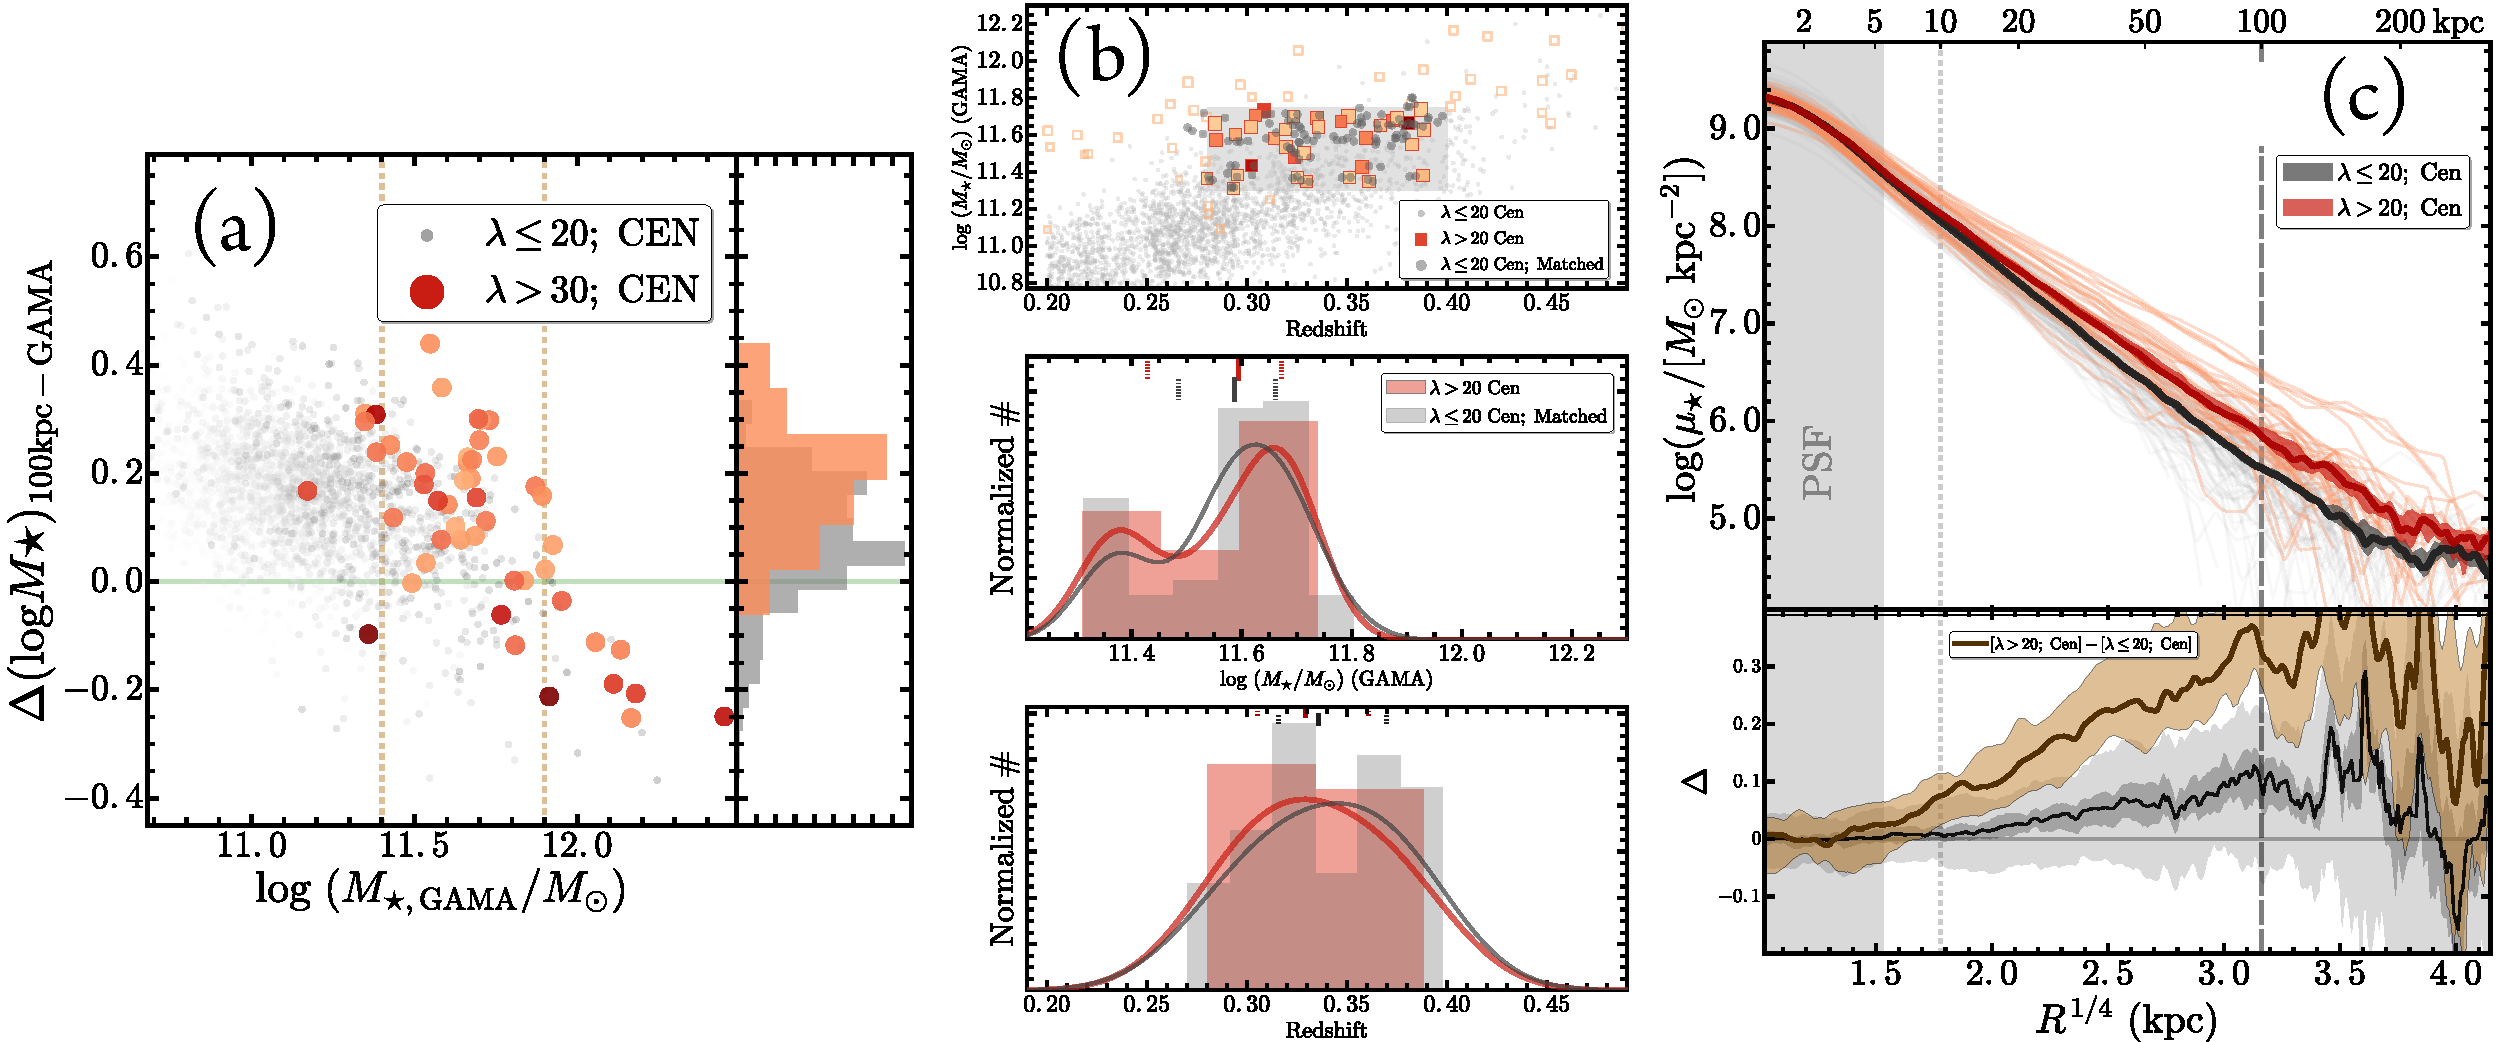
\includegraphics[width=\textwidth]{fig/redbcg_prof_gama_new}
    \caption{
        \textbf{Left:} comparison of \mstar{} estimated by the GAMA survey and 
        the \mtot{} using HSC images in this work. 
        We plot the \logmgama{} against the difference between \logmtot{} and \logmgama{}. 
        The format is very similar to the left panel of Fig~\ref{fig:smf1}. 
        The two vertical lines highlight the mass range $11.4 \leq$\logmgama{}$<11.8$ 
        that is used for the comparison.~~
        \textbf{Right:} we compare the \mden{} profiles of \rbcg{} (orange-red) and 
        \nbcg{} (grey-black) galaxies using the samples matched on the 
        \mgama{}-$z$ plane at $11.4 \leq$\logmgama{}$<11.9$ and $0.28 \leq z < 0.4$. 
        The format is very similar to the ones in Fig~\ref{fig:prof_1}.}
    \label{fig:gama}
\end{figure*}
%% ------------------------------------------------------------------------------------ %% 

    The GAMA survey greatly overlaps with the HSC survey, and it provides carefully 
    measured \mstar{} for large sample of galaxies (\citealt{Taylor2011}) that help 
    produce many interesting results (e.g. \citealt{Bauer2013, Ferreras2017}).
    They use 2-D single-\ser{} model to correct the total luminosity of the galaxy 
    (\citealt{Kelvin2012}), and derive the \m2l{} through optical-SED fitting 
    (BC03 model; Chabrier IMF) based on the PSF-matched aperture photometry. 
    Since the \ser{} model is generally more flexible than the \texttt{cModel} one, 
    it is therefore interesting to compare with the \rbcg{} and \nbcg{} galaxies 
    that also have spec-$z$ (at $z < 0.40$) and \mstar{} in GAMA DR2 
    (\citealt{Liske2015}) and see the impact of deep photometry again. 
    
    We summarize the results in Fig~\ref{fig:gama}.  
    On the left panel, we compare the differences between \mtot{} and \mgama{}. 
    HSC survey on average recovers more \mstar{} at high-\mstar{} end, which is 
    consistent with the expectation from deeper photometry, although the 
    systematic differences in the estimates of \m2l{} could play a role here. 
    Meanwhile, it is interesting see that, above \logmtot{}$> 11.8$, \mgama{} 
    becomes increasingly larger than \mtot{}, and most of these massive 
    galaxies have very high \ser{} index from the 2-D fitting. 
    This suggests that the single-\ser{} model is no longer an appropriate one to 
    describe very massive galaxies as it tends to over-estimate the \mstar{} the 
    inner and/or outer regions. 
    
    To verify the cause of the difference in \mstar{}, we further select samples 
    of \rbcg{} and \nbcg{} galaxies with matched \mgama{} and redshift 
    distributions (at $11.4 <$\logmgama{}$<11.8$; see Appendix \ref{app:match}), 
    and compare their \mden{} profiles (right panel). 
    Although these two subsamples are equally massive according to results from 
    GAMA survey, it is clear that the \rbcg{} galaxy has much more extended 
    outer envelope, even though its median \mden{} profile is very similar 
    to the \nbcg{} sample at $< 10$ kpc. 
    We can reproduce very the same trend with the luminosity density profiles 
    (with or without $k$-correction), suggesting that the inaccurate \ser{} 
    model definitely leads to under-estimate of \mstar{}.  
 
%% ------------------------------------------------------------------------------------ %% 

\section{C. Comparisons of \mden{} profiles in different redshift bins}
    \label{app:redshift}

%% ------------------------------------------------------------------------------------ %% 
\begin{figure}
    \centering 
    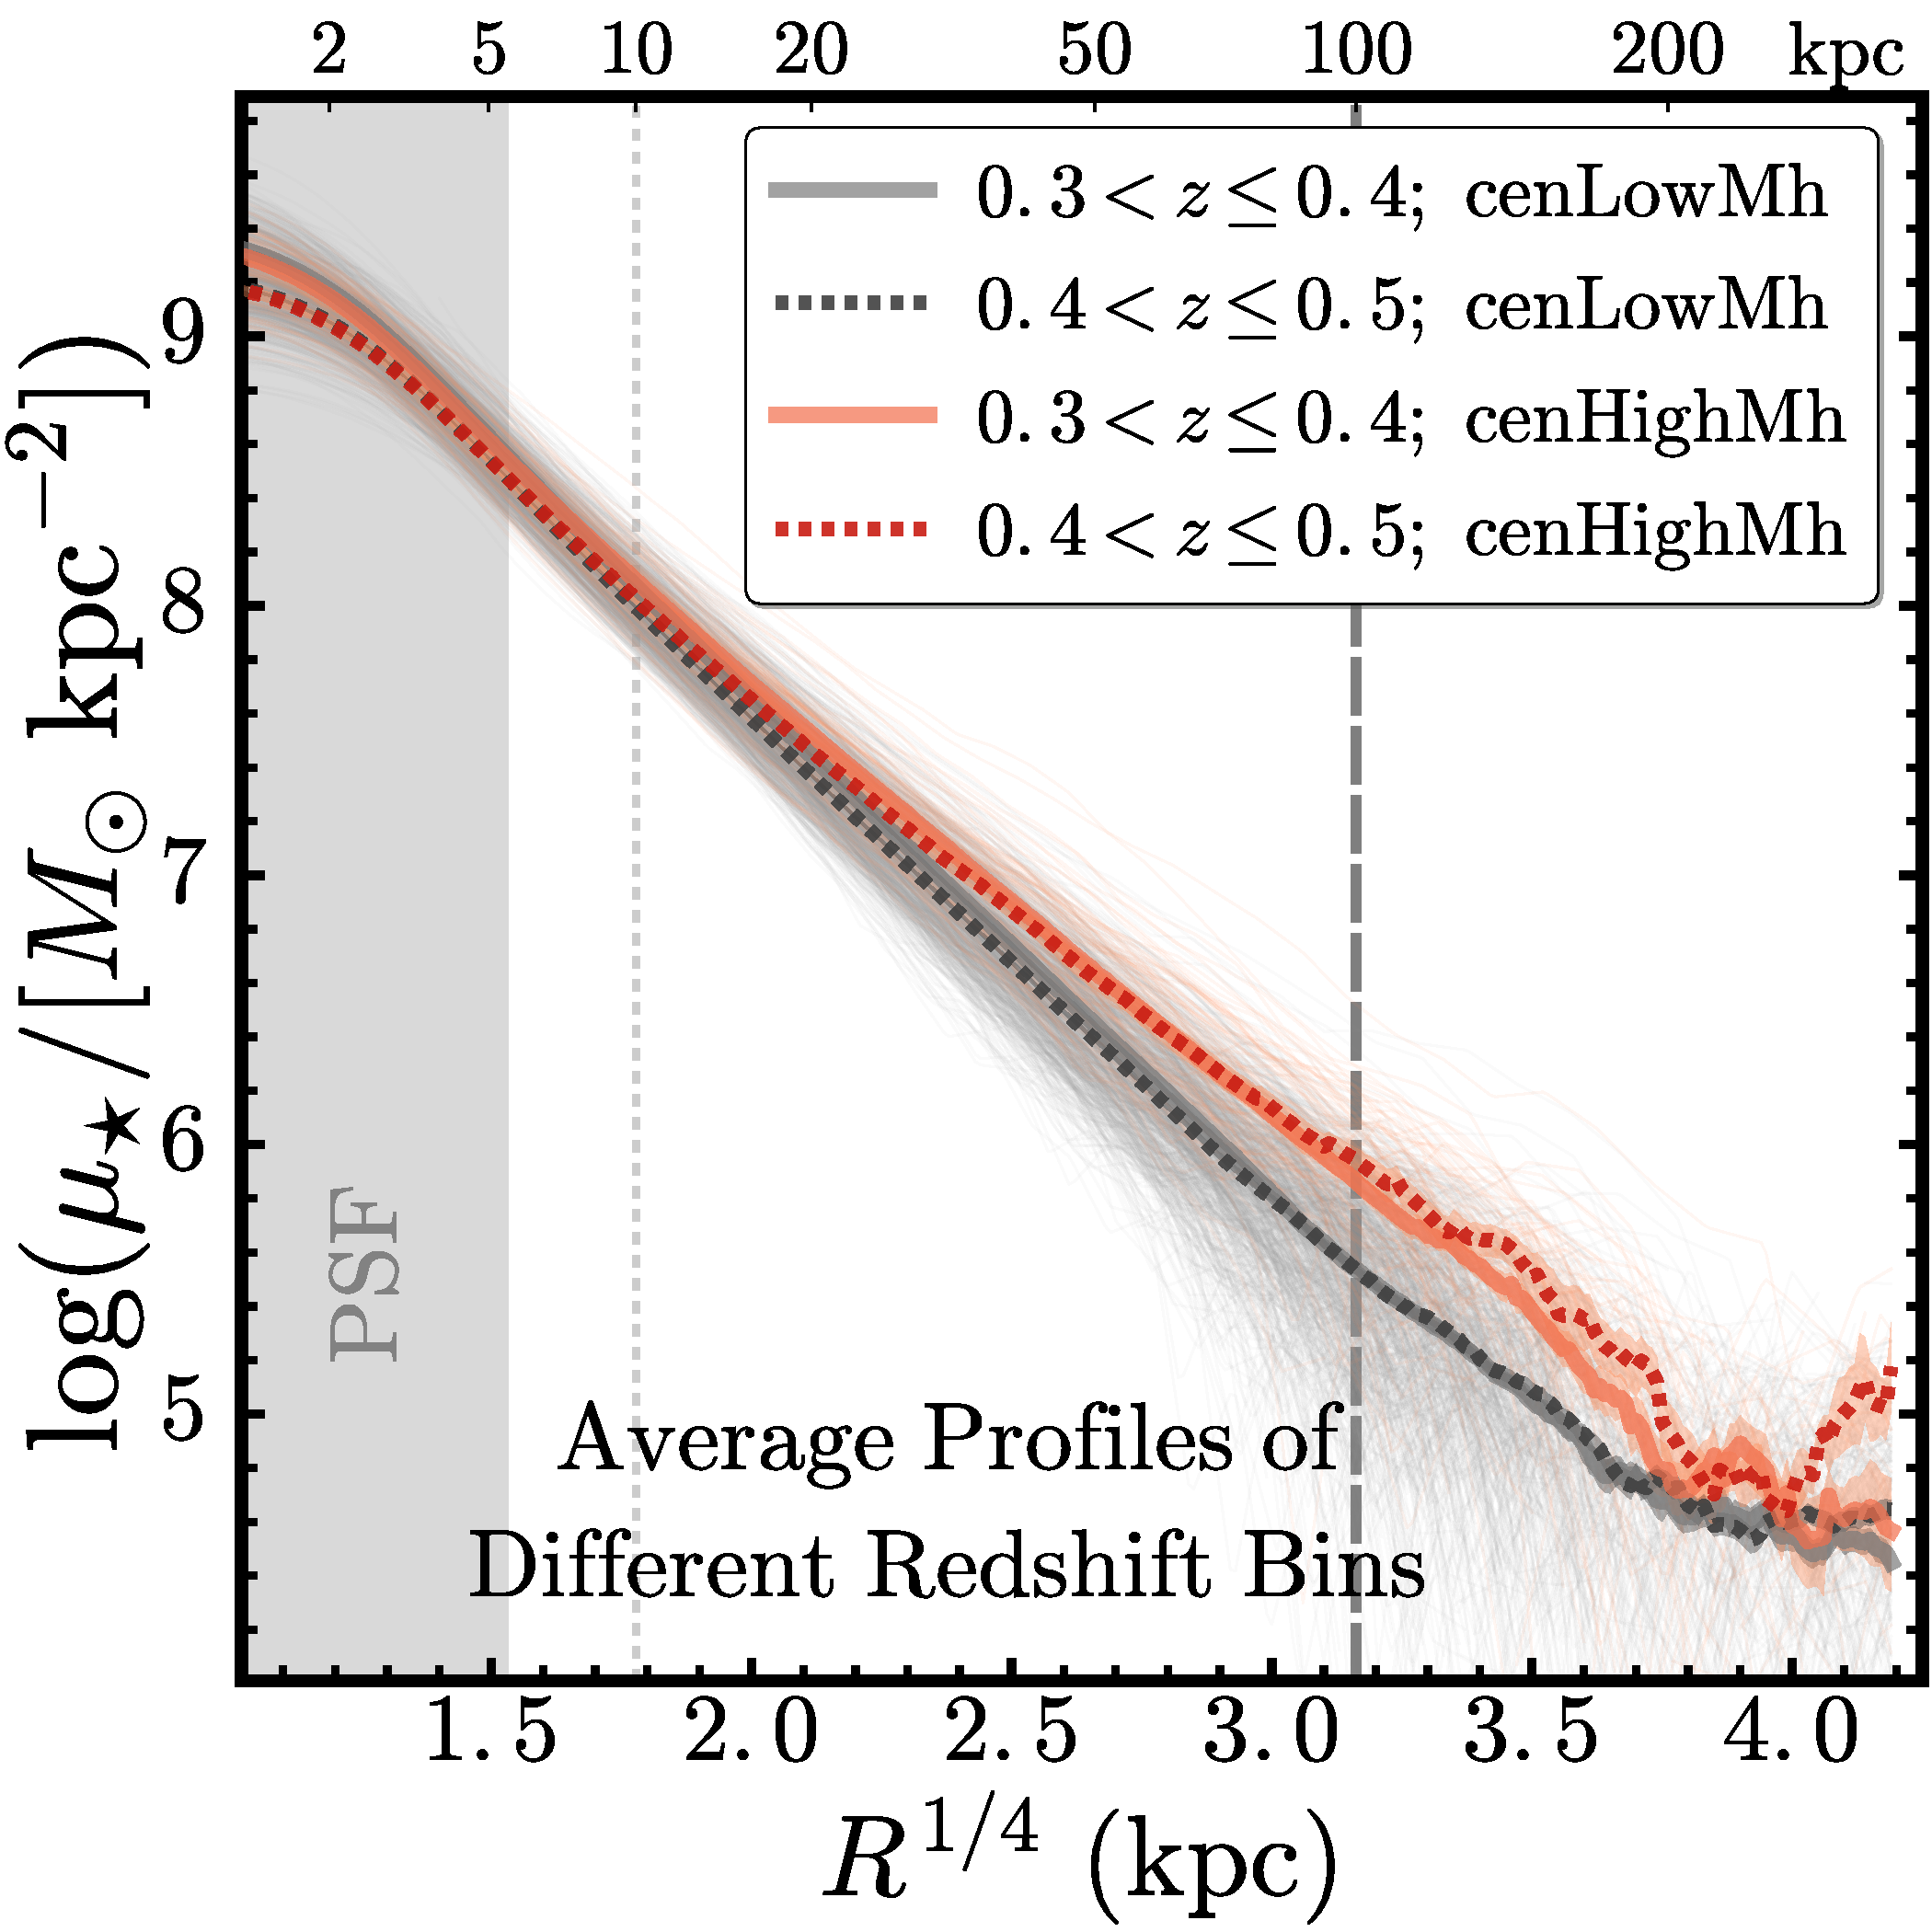
\includegraphics[width=8.2cm]{fig/redbcg_avg_prof_z}
    \caption{
        Comparison of \mden{} profiles of \rbcg{} (orange-red) and \nbcg{} 
        (grey-black) at $11.6 \le$\logmtot$< 11.9$ in redshift bins of 
        $0.3\leq z<0.4$ (solid lines) and $0.4\leq z<0.5$ (dash lines). 
        We show the individual profile in the background using much thinner line, 
        and highlight the median profiles using thicker line and darker color.
        Other formats are exactly the same with the left figure of 
        Fig~\ref{fig:avg_prof}.}
    \label{fig:avg_prof_z}
\end{figure}    
%% ------------------------------------------------------------------------------------ %% 
    
    Given the redshift range for our samples, it is important to evaluate 
    the impacts from the physical extend of seeing and the imaging depth on the \mden{} 
    profiles at different redshift. 
    Under the same seeing, the \mden{} profile of galaxy at higher-$z$ is more 
    vulnerable to the PSF smearing effect at the center. 
    It is also harder to reach to the same \mden{} level under the same imaging depth 
    due to cosmological dimming and background noise. 
    
    In Fig~\ref{fig:avg_prof_z}, we group the \rbcg{} and \nbcg{} galaxies within 
    $11.6 \le$\logmtot$< 11.9$ into two $z$ bins ($0.3\leq z<0.4$ and $0.4\leq z<0.5$),
    and compare their \mden{} profiles. 
    In two redshift bins, the median \mden{} profiles from the same sample follow each 
    other very well outside 10 kpc, but become visibly different in the central 3-4 kpc,
    where the effect from seeing kicks in. 
    Meanwhile, the median \mden{} profiles of \rbcg{} and \nbcg{} in the same $z$ bin 
    are identical in the central region, which indicates similar average seeing 
    conditions.       
    This confirms that \mden{} profile at $> 5$ kpc is safe from the impacts of seeing 
    and difference in redshift.
    More importantly, it also suggests that, once the redshift distributions are 
    carefully matched, the difference of \mden{} profile is likely to be physical 
    even in the central region.  

%% ------------------------------------------------------------------------------------ %% 

\section{D. Match the \rbcg{} and \nbcg{} samples in \mstar{} and redshift distributions}
    \label{app:match}

%% ------------------------------------------------------------------------------------ %% 
\begin{figure*}
    \centering 
    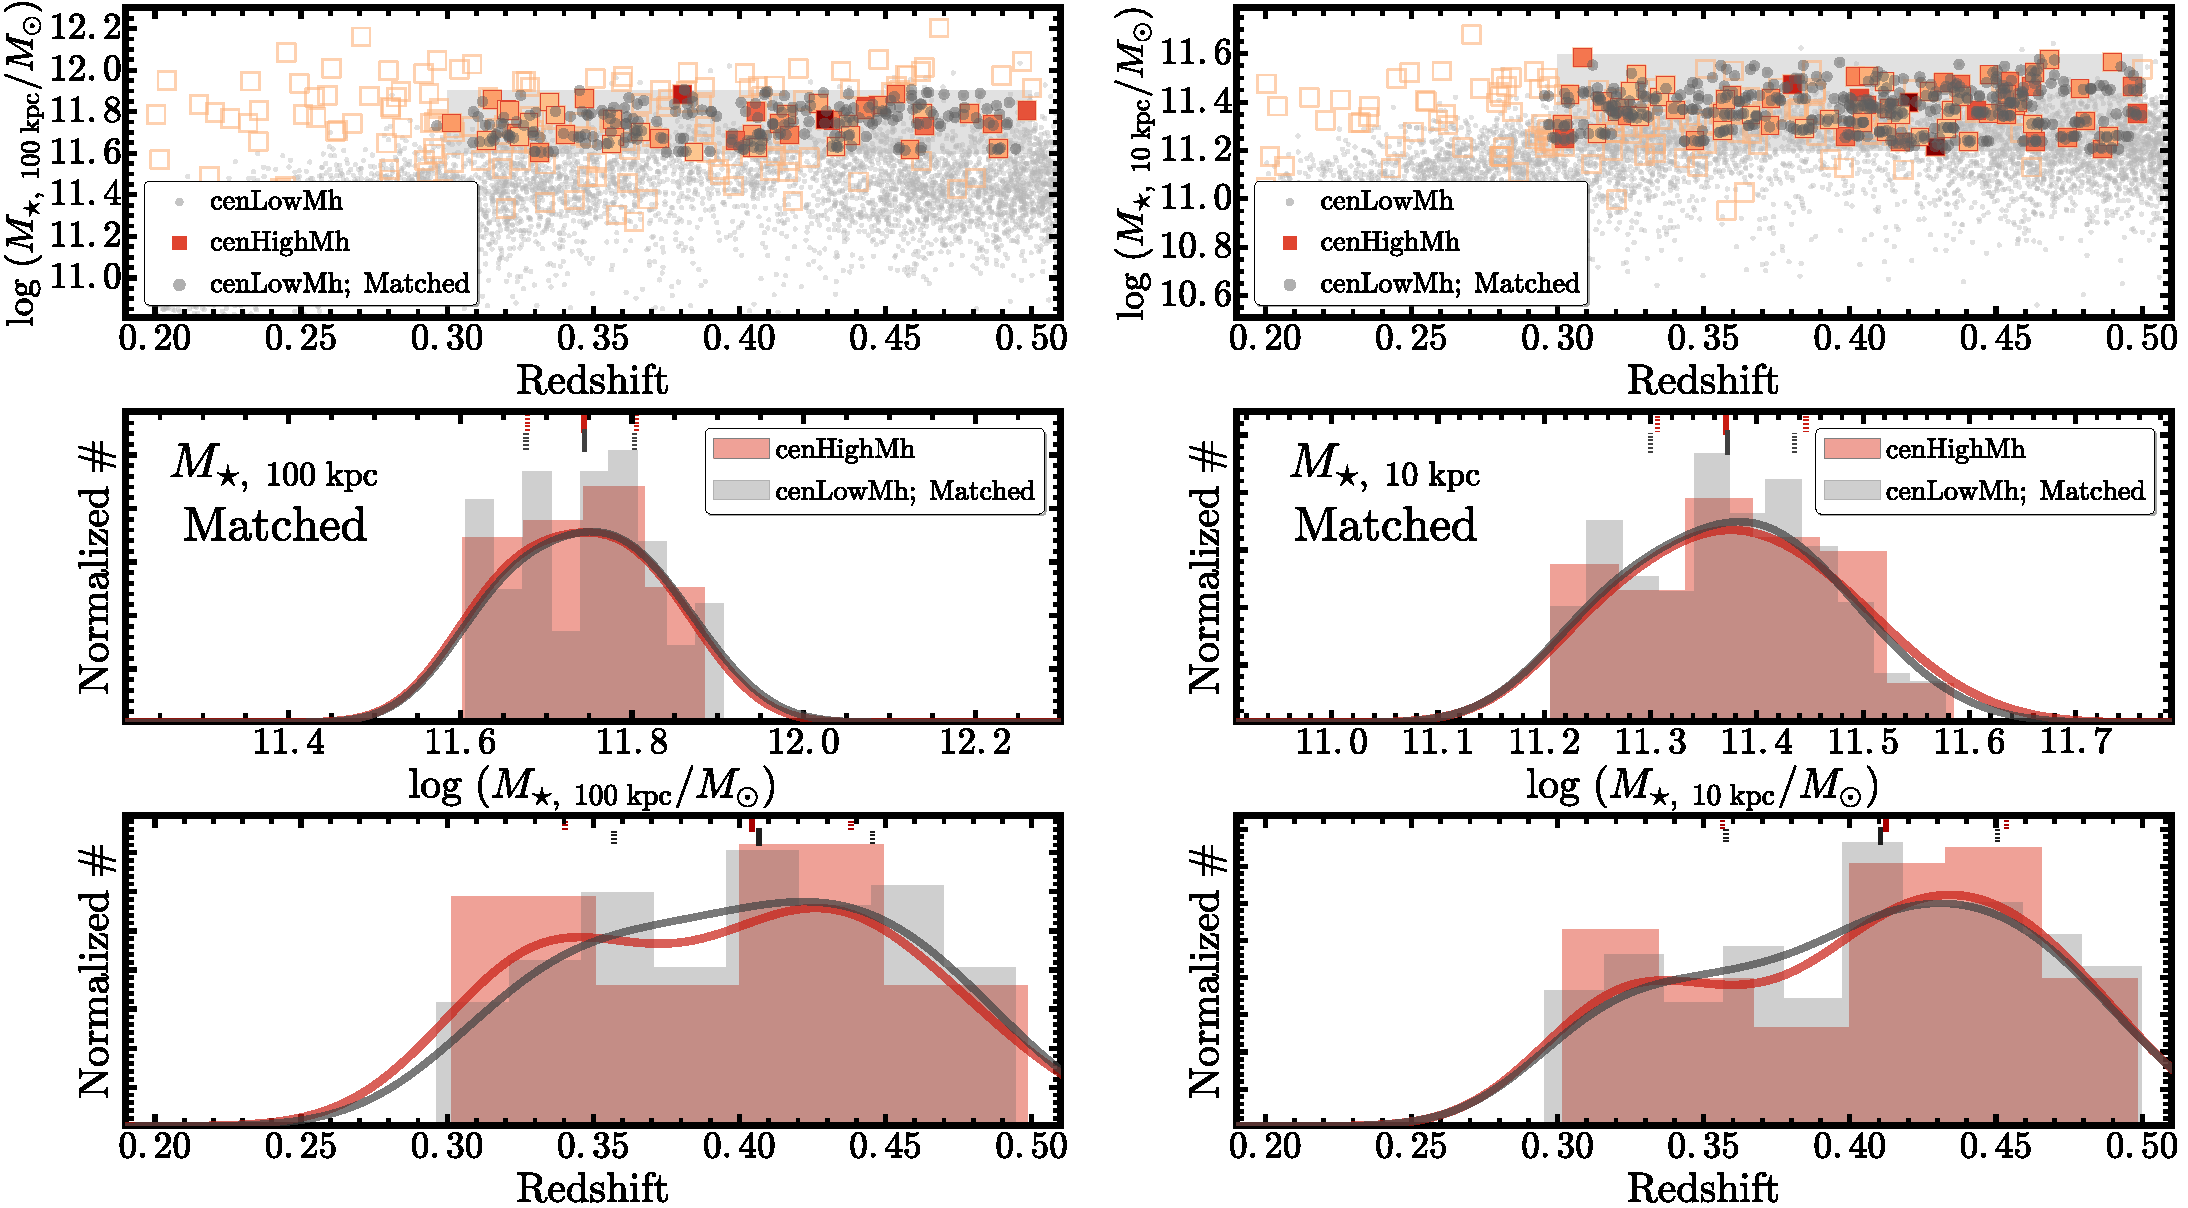
\includegraphics[width=\textwidth]{fig/redbcg_match}
    \caption{
        \textbf{Left figure} shows the details of the \mtot{}-matching process, 
        corresponding to the results shown in the left figure of   
        On the top panel, we show the overall distributions of \rbcg{} (light orange boxes) 
        and \nbcg{} (light grey dots) galaxies on the \mtot{}-$z$ plane.  
        And, we match the two sample in the \mtot{}-$z$ space outlined by the shaded region.
        We highlight the \rbcg{} galaxies in this region using bigger boxes in red frames, 
        whose size reflects the $P_{\mathrm{Cen}}$ value.  
        We also color-code them using the richness ($\lambda$) of the host cluster. 
        The matched \nbcg{} galaxies are highlighted using darker color and bigger dots. 
        To further evaluate the matching results, we show the distributions of \mtot{} 
        (middle panel) and redshift (bottom panel) separately. 
        On both panesl, we show the histograms along with their kernel density 
        distributions.  
        And, on the top of each panel, two sets of short vertical lines highlight the median 
        value (solid) and the inter-quartile (dash) of each distribution.~~~
        \textbf{Right figure} shows the similar matching results for the \minn{}-matched
        samples used for the right figure of Fig~\ref{fig:prof_1}.
        The format is exactly the same as the left one, except the \minn{} replaces the 
        \mtot{} in the top and middle panels.}
    \label{fig:match}
\end{figure*}
%% ------------------------------------------------------------------------------------ %% 
    
    As explained earlier, it is important to make sure the two samples have similar 
    distributions in both \mstar{} and redshift before comparing their median \mden{} 
    profiles.  
    Here we briefly describe the procedure used in this work. 
    Since the \rbcg{} sample is smaller in size, we always match the \nbcg{} sample to 
    it by searching for the $N$-nearest neighbours on the $M_{\star}$-redshift plane 
    using the KDTree algorithm in the \texttt{scikit-learn} Python library 
    (\citealt{scikit-learn}), and evaluate the quality of the match using the 
    distributions of both parameters (as shown in Fig~\ref{fig:match}). 
 
    As we only keep the unique \nbcg{} galaxies in the matched sample, we manually 
    adjust the value of $N$ to achieve the best match. 
    When the redshift distribution of the \rbcg{} sample becomes bi-model, we also try 
    to split the sample into two redshift bins and match them separately. 
    Typically $N$ is between 3 to 8.
    In Fig~\ref{fig:match}, we demonstrate this procedure using the results for 
    the \mtot{}-matched (Left) and the \minn{}-matched samples in Fig~\ref{fig:prof_1}
    (Right), and the two samples are well matched in the distributions of \mtot{}
    (or \minn{}) and redshift.  
    For all the comparisons of \mden{} profiles in this work, we match the samples 
    in the same way, and make sure the match has the same quality. 
    
%% ------------------------------------------------------------------------------------ %% 
\section{E. Robustness of the \mden{} Differences} 
	\label{app:robust}
    
    In Fig~\ref{fig:prof_1}, we compare the \mden{} profiles of \mtot{}- and 
    \minn{}-matched samples of \rbcg{} and \nbcg{} galaxies, and here we test the 
    robustness of the results using a few extra tests that are illustrated in
    Fig~\ref{fig:prof_2}, Fig~\ref{fig:prof_3}, and Fig~\ref{fig:prof_4}, and 
    are briefly described here:   
    
    \begin{enumerate}
        
        \item In Fig~\ref{fig:prof_2}, we group the samples into two \mtot{} bins. 
            Given the small sample size, we extend slightly toward lower \mtot{} range 
            ($11.5 \leq \log (M_{\star,\ 10\mathrm{kpc}}/M_{\odot}) < 11.7$ and 
             $11.7 \leq \log (M_{\star,\ 10\mathrm{kpc}}/M_{\odot}) < 11.9$). 
            Although the smaller sample leads to larger statistical uncertainties, 
            we can still see similar structural differences in both \mtot{} bins, 
            and the difference becomes more significant in the higher \mtot{} bin.  
            For the lower \mtot{} bin, the difference in the inner region becomes 
            quite uncertain, while the difference in the outskirt is still visible. 
            This potentially suggests that the environmental dependence of structure 
            also varies with \mstar{}, an important implication deserves more 
            investigations in the future.   

        \item On the left panel of Fig~\ref{fig:prof_3}, we match the \rbcg{} and 
            \nbcg{} samples in a lower redshift bins ($0.30 < z < 0.42$).
            Despite the larger uncertainties due to smaller samples, we find the 
            results are the same.
            
        \item On the middle panel of Fig~\ref{fig:prof_3}, we includes \rbcg{} 
            galaxies in poorer clusters ($20 < \lambda < 30$), which should result 
            in overlapped \mhalo{} distributions with the \nbcg{} samples 
            considering the typical uncertainty of $\lambda$.
            This makes the difference in the inner region slightly less significant, 
            but the overall results are the same. 
             
        \item On the right panel of Fig~\ref{fig:prof_3}, in stead of using \mtot{}, 
            we use the \mmax{}--the maximum \mstar{} by integrating the \mden{} 
            profiles to the largest radius allowed.  
            The \mmax{} values are less reliable than \mtot{} due to the 
            uncertainty of background subtraction and contamination from nearby 
            bright objects, but they can serve as different estimates of the ``total''
            \mstar{} of these galaxies.
            As shown in Section~\ref{sec:discussion}, they on average increase
            the \mstar{} by a little bit and affect the \rbcg{} more.
            The differences in the \mden{} profiles still remain very similar.
      
    \end{enumerate}
    
    We also test the robustness of the \mtot{}-matched results using the samples with 
    only spectroscopic redshift, the samples in the three GAMA fields, and the \rbcg{} 
    samples without the ones in very massive haloes ($\lambda > 40$).  
    Limited by space, we do not show these results here, but they all verify the 
    robustness of the results. 
    
    For the results from the \minn{}-matched samples: 
    
    \begin{enumerate}
    
        \item
            We match the two samples using both \minn{} and the \mstar{} within 15 kpc 
            at the same time.  
            This makes the two median \mden{} profiles very similar inside 10-15 
            kpc, while the result in the outskirt remains the same (left panel of 
            Fig~\ref{fig:prof_4}).
            Use \mstar{} within 5 or 20 kpc leads to the same conclusion. 
          
        \item 
            To make sure the two samples are comparable in their overall assembly history,
            we also try to only include the very massive galaxies (\logmtot{}$>11.5$)
            in both samples. 
            This excludes the \nbcg{} galaxies that are much less massive and 
            more ``compact'' in structure. 
            Yet, the results regarding the structural differences remain the same. 
          
    \end{enumerate}

%% ------------------------------------------------------------------------------------ %% 
  \begin{figure*}
      \centering 
      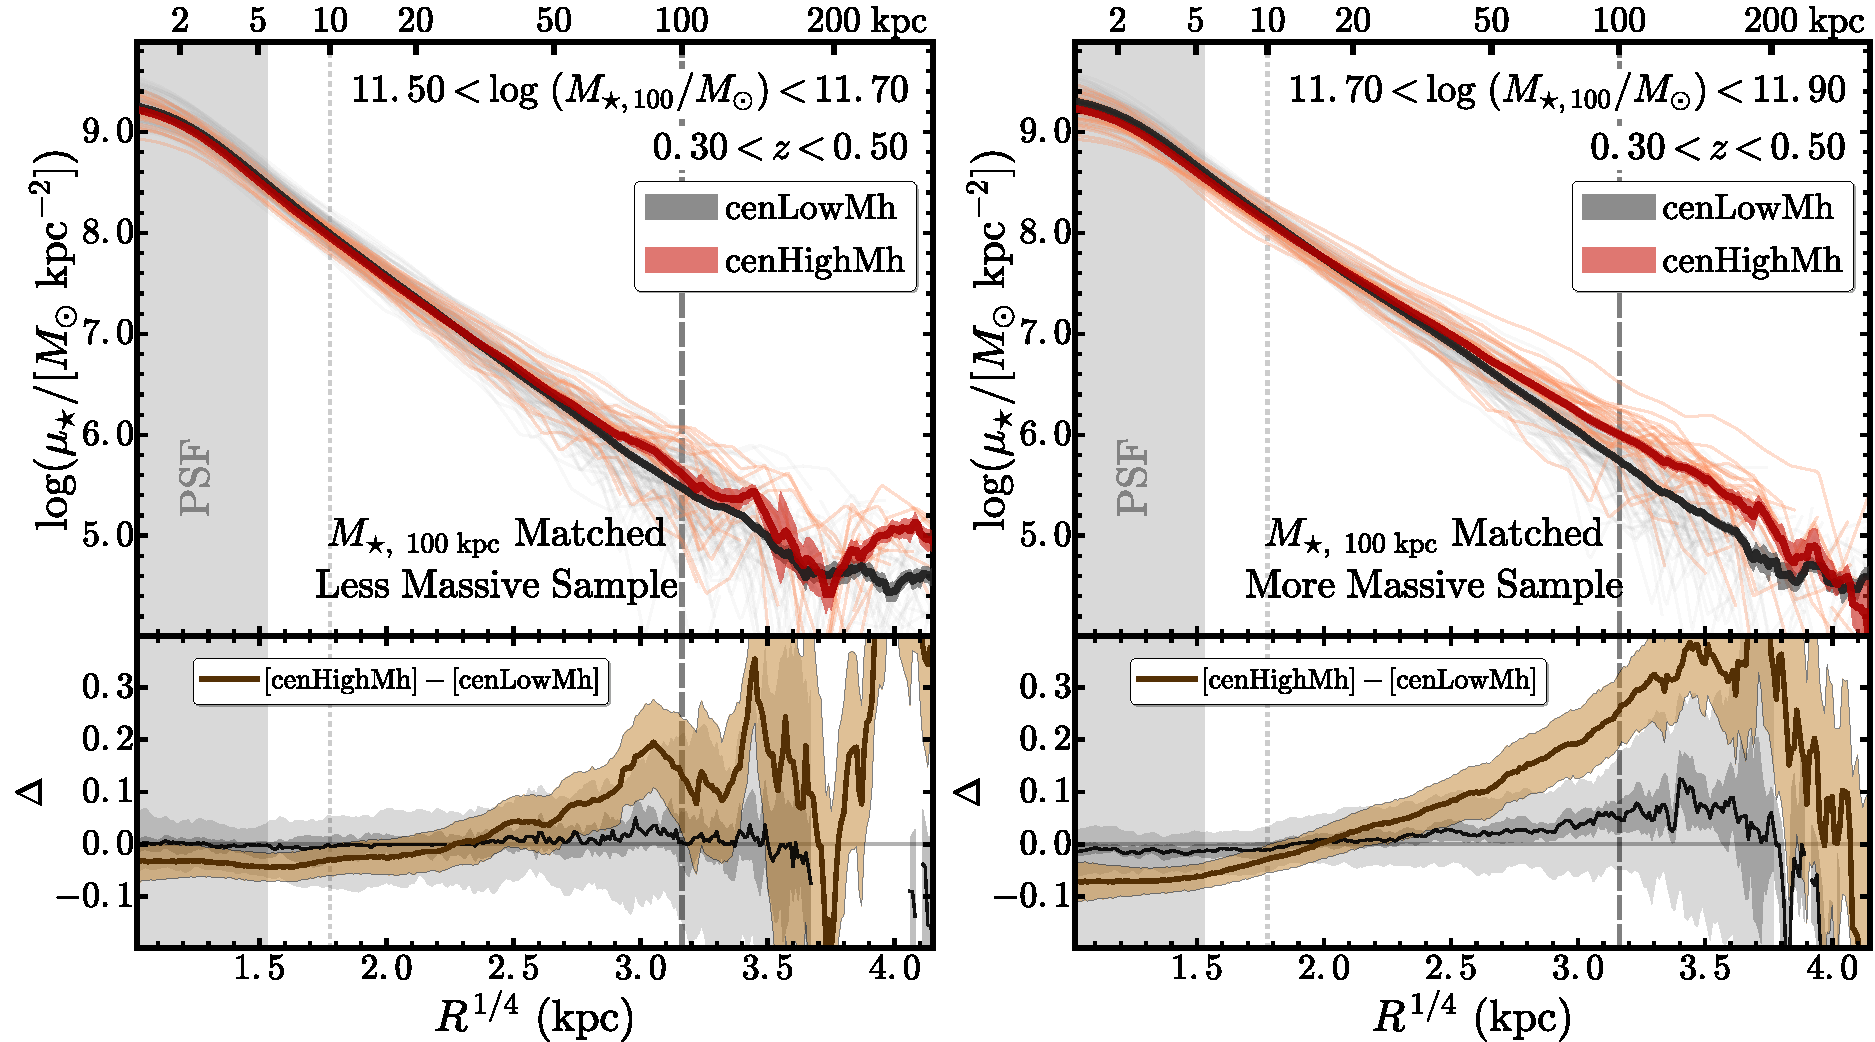
\includegraphics[width=\textwidth]{fig/redbcg_prof_2}
      \caption{
          Comparisons of the \mden{} profiles for \mtot{}-matched \rbcg{} 
          (orange-red) and \nbcg{} (grey-black) galaxies in lower (left; [11.5,11.70]) 
          and higher (right; [11.7, 11.9]) \mtot{} bins. 
          Other formats are in consistent with the right figure of Fig~\ref{fig:prof_1}.
          The difference in median profiles is more significant in higher \mtot{} bin.
          }
      \label{fig:prof_2}
  \end{figure*}
%% ------------------------------------------------------------------------------------ %% 

%% ------------------------------------------------------------------------------------ %% 
  \begin{figure*}
      \centering 
      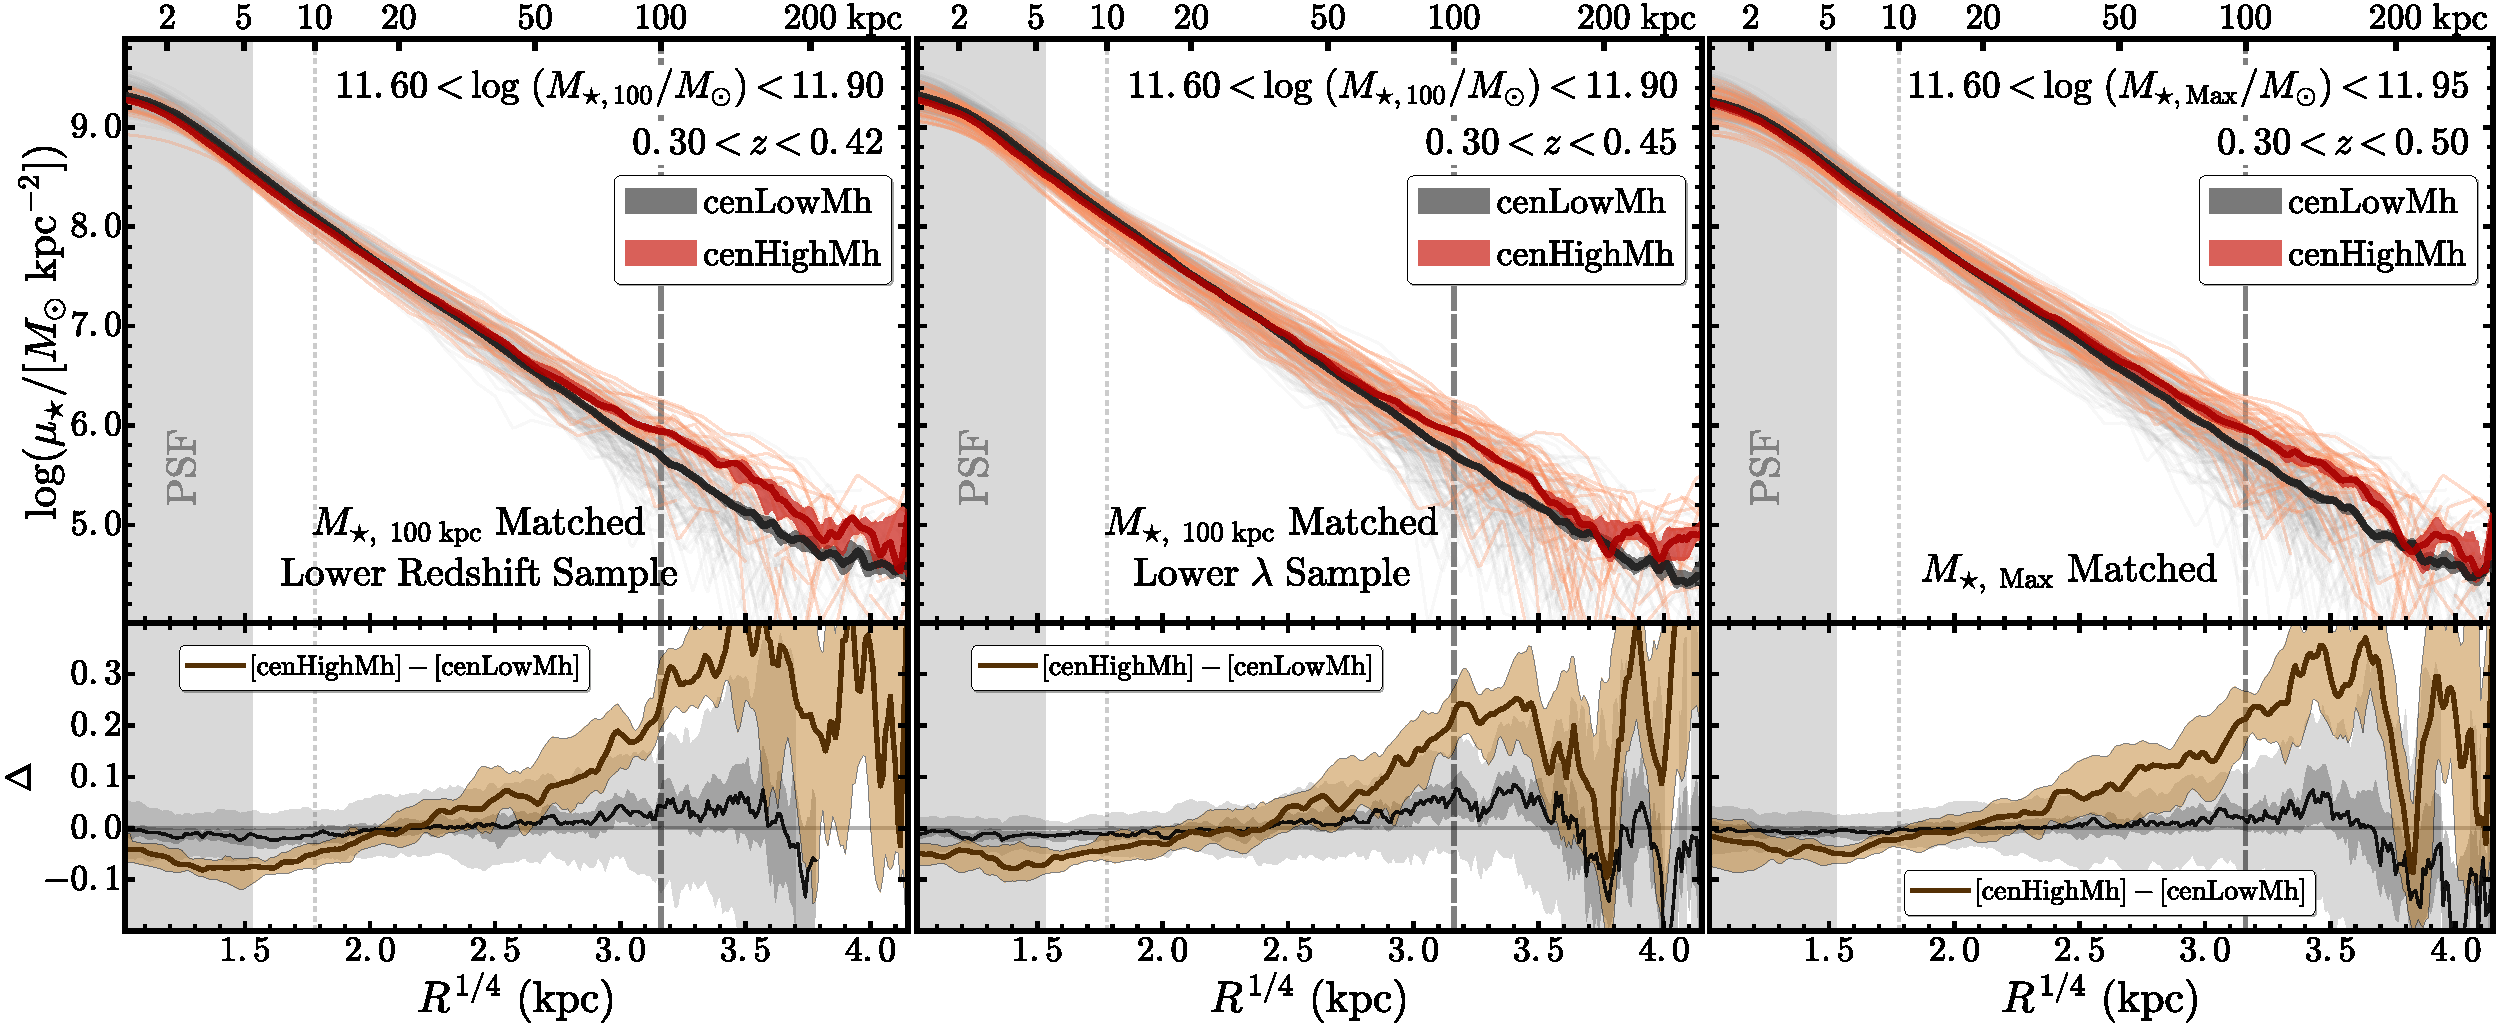
\includegraphics[width=\textwidth]{fig/redbcg_prof_3}
      \caption{
        Comparisons of the \mden{} profiles for \rbcg{} (orange-red) and \nbcg{} 
      	(grey-black) galaxies that are matched using proxies of total \mstar{}. 
        The formats are in consistent with the right figure of Fig~\ref{fig:prof_1}.
        The differences are, here, the samples are matched in slightly differnt ways. 
        From left to right: a) using samples at lower redshift ($0.3 < z < 0.4$); 
        b) using \rbcg{} sample with $\lambda > 20$ instead of 30; 
        c) using \mstar{} within 150 kpc instead of 100 kpc.
        The results are broadly consistent with the one in Fig~\ref{fig:prof_1}.
        }
      \label{fig:prof_3} 
  \end{figure*}
%% ------------------------------------------------------------------------------------ %% 

%% ------------------------------------------------------------------------------------ %% 
  \begin{figure*}
      \centering 
      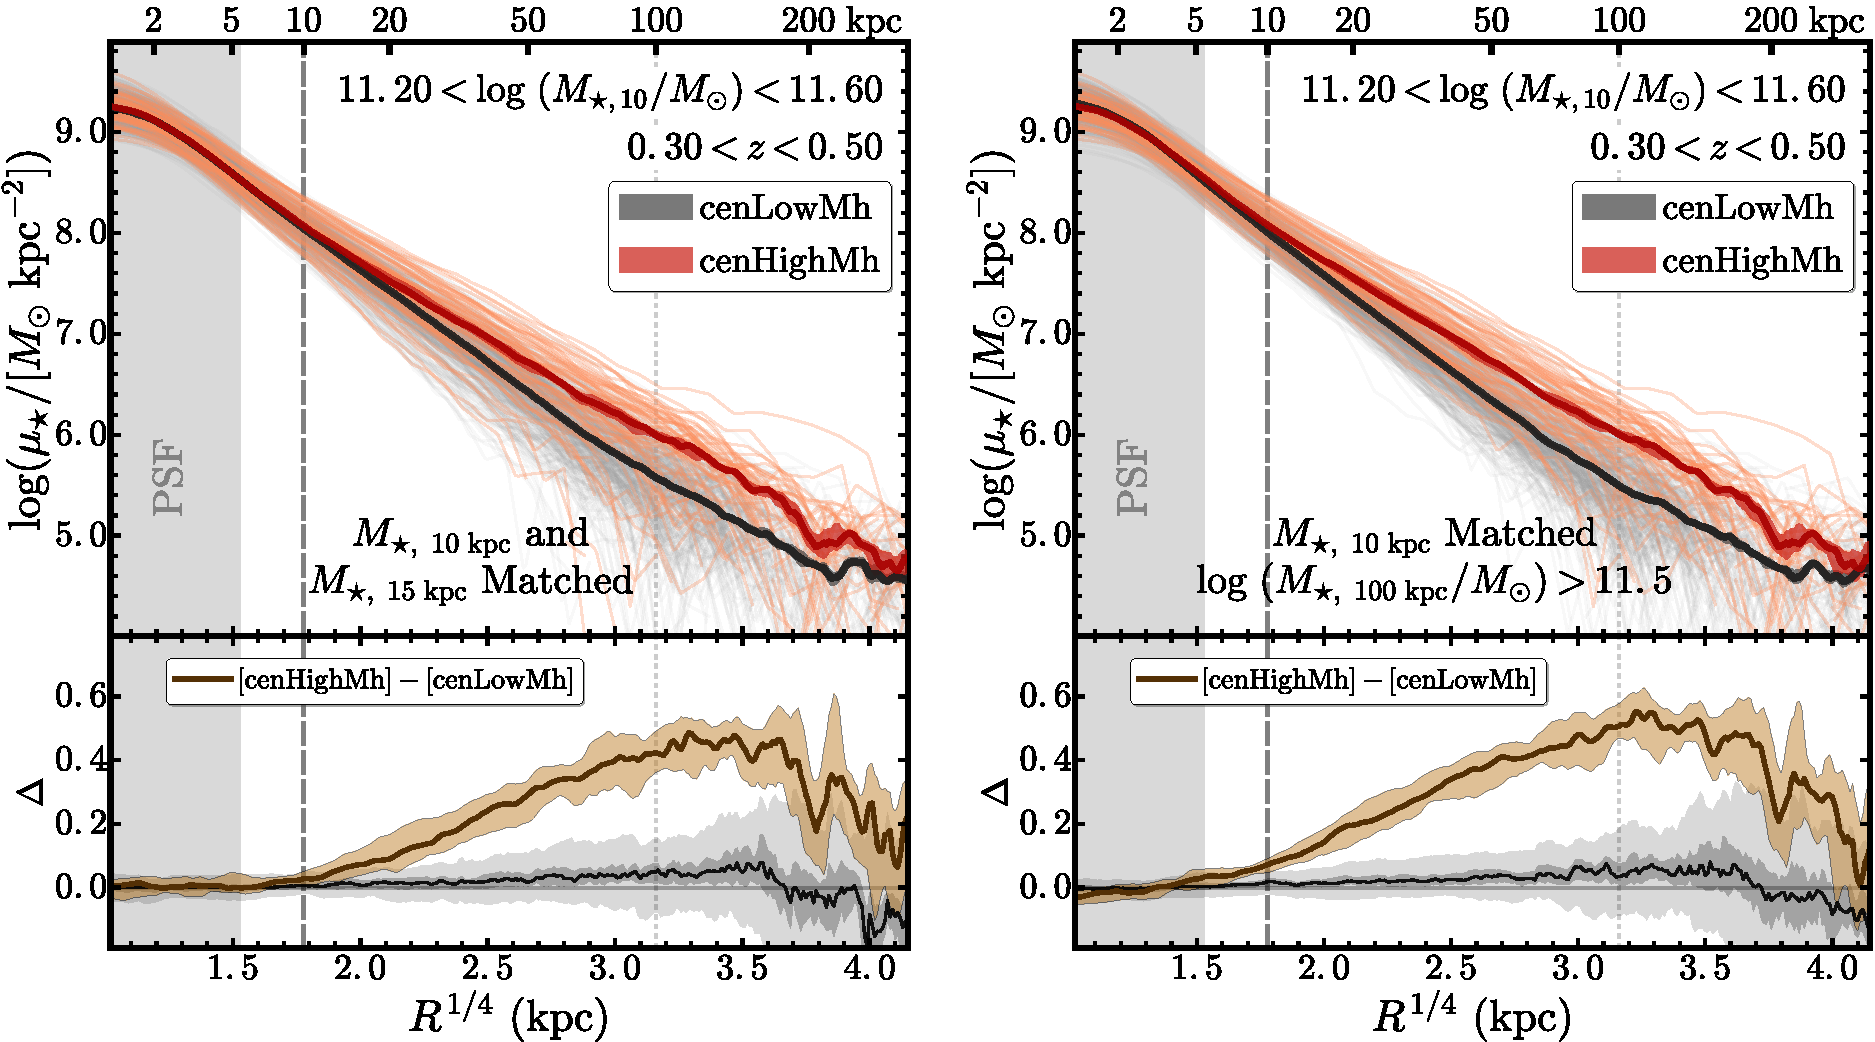
\includegraphics[width=\textwidth]{fig/redbcg_prof_4}
      \caption{
          Comparisons of the \mden{} profiles for \rbcg{} (orange-red) and \nbcg{} 
          (grey-black) galaxies that are matched using the \mstar{} enclosed in the 
          inner region. 
          Left panel shows the results after matching the \minn{} and \meff{} together, 
          and the right panel shows the results when only the \logmtot{}$\ge 11.5$
          \rbcg{} and \nbcg{} galaxies are included.
          Other formats are in consistent with the right figure of Fig~\ref{fig:prof_1}.
          }
      \label{fig:prof_4} 
  \end{figure*}
%% ------------------------------------------------------------------------------------ %% 

%% ------------------------------------------------------------------------------------ %%  
\bsp
\label{lastpage}
\end{document}
%% ------------------------------------------------------------------------------------ %% 
%%%%%%%%%%%%: End of the File %%%%%%%%%%%%
%% ------------------------------------------------------------------------------------ %% 